%************************************************
\chapter{Lightly Ionizing Particle Search}

\label{ch:lips} % $\mathbb{ZNR}$
%************************************************

\begin{flushright}{\slshape    
   And all this science I don't understand, \\
     It's just my job five days a week. } \\ \medskip
    --- {Elton John, \textit{Rocket Man, 1972}}
\end{flushright}

\section{LIP Search with LUX}
This chapter details the search for \ac{LIP}s in the \ac{LUX} detector during Run03. Recall from Chapter~\ref{ch:theory} that \ac{LIP}s are present in some hidden sector models, and may comprise some part of the dark matter density observed today. \ac{LIP}s carry an effective fractional charge, $e/f$, in their interactions with visible matter. Depending on the charge and mass of such a particle, it could precess along the galactic magnetic field lines and be carried out of the galactic disk \cite{McDermott2011}. This effect would make direct detection on Earth of relic \ac{LIP}s over a region of mass-charge space very difficult. Therefore, we limit the \ac{LIP} search to cosmogenic \ac{LIP}s which can be created in the upper atmosphere or in high energy astrophysical events; such interactions are also capable of producing \ac{LIP}s with masses inaccessible to collider experiments \cite{Agnese2015}. Searches for cosmogenic \ac{LIP}s were carried out by Kamiokande II \cite{Mori1991}, MACRO \cite{Ambrosio2000} \cite{Ambrosio2004}, and LSD \cite{Aglietta1994} for a charge range between $1$ and $e/5$. The cryogenic germanium detectors CDMS \cite{Agnese2015} and the Majorana Demonstrator \cite{Alvis2018} carried out searches in the charge range $\leqslant e/6$. Each of these searches is summarized briefly in Chapter~\ref{sec:dm_detection_schemes}. All of these previous searches set limits on the flux as a function of charge fraction, $f$; they do not set limits on \ac{LIP} mass, as the interaction cross section is independent of mass and depends very strongly on charge, scaling as $1/f^{2}$ (see below in Section~\ref{sec:pai}). The flux $\Phi$ is defined as:

\begin{equation}
\label{eq:flux}
\Phi = \frac{n}{A t \epsilon \Omega}
\end{equation}
where $A$ is the cross-sectional area of the detector, $t$ is the time over which the search was carried out, $\epsilon$ is the detection efficiency, and $\Omega$ is the solid angle, or geometrical efficiency of the detector.

Previous cosmogenic \ac{LIP} searches, as well as the one presented here, make the following assumptions:

\begin{itemize}
\item \ac{LIP}s are cosmogenic.
\item The incident distribution is isotropic in the upper 2$\pi$ and 0 below.
\item \ac{LIP}s are relativistic, and therefore do not deviate from a straight path as they pass through the detector.
\item \ac{LIP}s are minimum ionizing. That is, their kinetic energy is such that they deposit the minimum amount of energy in the detector.
\end{itemize}

The last assumption, that \ac{LIP}s are minimum ionizing, is the most conservative assumption that can be made about \ac{LIP} energy. There is no theoretical \ac{LIP} energy spectrum. Any other (greater) energy loss would increase the detection efficiency, making the experiment more sensitive. Assuming minimum ionizing energy loss will generally give the least restrictive limit in the absence of a discovery. It should be noted that there is not a particular motivation that the incident spatial distribution be isotropic in the upper 2$\pi$, but that is the practice that \ac{CDMS} and \ac{MJD} follow.


\section{Modeling LIP Interaction}
This section describes the steps to modeling \ac{LIP} interactions for a wide range of \ac{LIP} charges in the \ac{LUX} detector to determine the detector response. 

\subsection{Collision Cross Section}
A \ac{LIP} interacting in the \ac{LXe} volume loses energy via interaction with electrons.  To model \ac{LIP}s in \ac{LUX}, the expression of interest is the collision cross section \ac{CCS}. The differential \ac{CCS} describes the energy lost to electrons in a single collision for incident energy of the LIP. For particles with charge $ze$ and mass M heaver than the electron mass$ m_{e}$ ( ``heavy'' particles are those with $M > m_{e}$), the Rutherford cross section is a familiar differential \ac{CCS} \cite{PDG}:

\begin{equation}
\label{ruth}
\frac{d\sigma_{R}}{dE} = \frac{2\pi r_{e}^{2} c^{2} z^{2}}{\beta^{2}} \frac{1-\beta^{2} E/ T_{max}}{E^{2}}
\end{equation}
where $r_{e}$ is the classical electron radius, $E$ is the energy loss of the incoming particle, $\beta = v/c$ is the velocity of the incoming particle, and $T_{max}$ is the maximum energy transfer possible in a single collision:

\begin{equation}
\label{Tmax}
T_{max} = \frac{ 2m_{2}c^{2} \beta^{2} \gamma^{2}}{1 + 2\gamma m_{e} / M + (m_{e}/M)^{2}}
\end{equation}
Often the expression $T_{max} = 2m_{e}c^{2} \beta^{2}\gamma^{2}$ for $2\gamma m_{e} / M<< 1$ is used implicitly, or is referred to as the ``low energy approximation'' in older texts. The Rutherford cross section is a good starting point, but it describes the ``hard interaction'' or head-on, billiard-ball type collision of a particle interacting with free electrons. Real electrons are bound in atoms, and an incident particle can undergo ``soft interactions'', in which virtual photons are exchanged. When the virtual photon matches the energy of electron orbitals of the target material, there are resonances in the \ac{CCS}. The energy transfer, $E$, must also be finite in real atoms, where the dielectric properties modify the electromagnetic field of a moving charged particle and limit the growth of the cross section. This real-world behavior is described by a correction factor $B(E)$, also sometimes called an ``inelastic form factor'' \cite{PDG}:

\begin{equation}
\label{totalccs}
\frac{d\sigma_{CCS}}{dE} = \frac{d\sigma_{R}}{dE} B(E)
\end{equation}
%Some of these can be found in [cite 18,27, 41-43 papers from Bichsel].
Various attempts spanning the 1900's have been made to take into account the real-world behavior of electrons bound in matter. The most well-known contributions are those of Bethe and Fano. In 1930, Bethe derived a cross section doubly differential in energy loss and momentum transfer using the first Born approximation for scattering on free atoms \cite{Bethe:1930}. In 1963, Fano extended the method to describe atoms in solids \cite{Fano:1963}. Combining their two methods yields the Bethe-Fano cross-section, which has undergone much study and by our current understanding has been verified to be close to reality \cite{Bichsel:2006}. There is another method, called the \ac{PAI} model, that is easier to calculate than the Bethe-Fano cross section, and approximates the Bethe-Fano calculation very closely \cite{Bichsel:2006}. This thesis uses the \ac{PAI} model as a base to determine energy deposition, building the full signal model for \ac{LIP}s interacting in the \ac{LUX} detector. 

\subsection{Photo Absorption Ionization Model for Charged Particle Energy Loss}
\label{sec:pai}
The \ac{PAI} model is also sometimes known as the \ac{FVP} or Weis\"{a}cker-Williams approximation. The generalized complex dielectric constant $\epsilon = \epsilon_{1} + i \epsilon_{2}$ can be thought of a encoding all the information about a medium. The real part $\epsilon_{1}$ describes the polarization of the material and imaginary part $\epsilon_{2}$ describes the absorptive properties. Typically both $\epsilon_{1}$ and $\epsilon_{2}$ are thought of as functions of $\omega$, or incident photon energy. In the case of inelastic collision, they are also functions of $k$, which denotes momentum transfer to atomic electron. So $\epsilon(\omega)  = \epsilon_{1}(\omega, k) + i \epsilon_{2}(\omega, k)$. The generalized dielectric constant $\epsilon(k, \omega)$ can be related to atomic matrix elements, and if desired, calculated completely and tediously. However, the \ac{PAI} model allows us to avoid these tedious calculations by making specific approximations.

In particular, the \ac{PAI} model approximates $\epsilon_{2}(k, \omega)$ by noting that typically, the momentum $k$ transferred to an electron is much less than the energy transfer $\omega$, and so the limit $k \rightarrow 0$ can be applied below some energy, and above that energy, electrons can be treated as quasi-free. A full derivation of the relativistic \ac{PAI} cross section can be found in \cite{AllisonCobb:1980}, and a useful summary is in \cite{Bichsel:2006}. Here, we quote the result:

\begin{equation}
\label{eq:pai}
\begin{split}
\frac{d\sigma_{PAI}(E; \beta)}{dE} &= \frac{\alpha}{\beta^{2} \pi} \frac{\sigma_{\gamma}(E)}{EZ} \mathrm{ln}[(1-\beta^{2}\epsilon_{1}(E))^{2} + \beta^{4}\epsilon_{2}(E)^{2}]^{-1/2} \\
&+ \frac{\alpha}{\beta^{2} \pi} \frac{1}{N \hbar c} \Big ( \beta^{2} - \frac{\epsilon_{1}(E)}{ | \epsilon(E) | ^{2}} \Big ) \theta \\
&+  \frac{\alpha}{\beta^{2} \pi} \frac{\sigma_{\gamma}(E)}{EZ} \mathrm{ln}\Big( \frac{2 m_{e}c^{2}\beta^{2}}{E} \Big) \\
&+  \frac{\alpha}{\beta^{2} \pi} \frac{1}{E^{2}} \int_{0}^{E} \frac{\sigma_{\gamma}(E^{\prime})}{Z} dE^{\prime} 
\end{split}
\end{equation}
where $N$ is the electron density in the medium (cm$^{-3}$) and $\sigma_{\gamma}$ is the photoabsorption cross section. Each of these terms is related to a physical phenomenon. The significance of these terms is described in detail in \cite{AllisonCobb:1980}; here we briefly summarize the salient points. The first two terms describe relativistic behavior, and the last two are the only present terms in non-relativistic theory. The natural logarithm in the first term is responsible for the relativistic rise in energy deposition. The second term describes the emission of Cherenkov radiation. The last two terms only have a $1/\beta^{2}$ dependence on velocity, and become effectively constant in the relativistic region. The third term describes resonance absorption at atomic energy levels, and the fourth term is the quasi-free region of Rutherford scattering, where electrons are treated as unbound.

%The first two terms are known as the transverse cross section, because they come from the magnetic vector potential term for which the electric field is transverse to the 3-momentum transfer. 
%The last two terms are known as the longitudinal cross section, because they come from the electrostatic term in the potential, which has the electric field parallel to momentum transfer.

While Equation~\ref{eq:pai} looks complicated, the convenience of this model lies in the fact that one need only obtain $\sigma_{\gamma}(E)$ or $\epsilon_{2}$ to carry out the calculation. This is because $\sigma_{\gamma}(E)$ is related to $\epsilon_{2}$ by:

\begin{equation}
\label{eq:sigma_gamma}
\sigma_{\gamma}(E) \sim \frac{E}{N} \epsilon_{2}
\end{equation}

and $\epsilon_{1}$ and $\epsilon_{2}$ are related by a Kramers-Kronig relation:

\begin{equation}
\epsilon_{1} - 1 = \frac{2}{\pi} P \int_{0}^{\infty} \frac{ x \epsilon_{2}(x)}{x^{2} - \omega^{2}} dx
\end{equation}
where P indicates the Cauchy principal value of the integral. Variable changes from $E$ to $\omega$ can be made the usual way: $E = \hbar \omega$. In practice, one does not find tabulated values of $\epsilon_{1}$, $\epsilon_{2}$, and $\sigma_{\gamma}$, but rather a variety of databases contain a variety of different optical constants. The optical constants can be related to $\epsilon_{1}$, $\epsilon_{2}$, and $\sigma_{\gamma}$ as needed. For this thesis, the same sources for optical constants as in the \ac{CDMS} \ac{LIP} result \cite{Prasad2013} were used. More detail along with tabulated values for the cross section can be found in Appendix~\ref{app:cross_section}. In general, high quality optical constants are desired because they greatly affect the result. Using the same sources as \cite{Prasad2013} for optical constants, the \ac{PAI} cross section was first calculated for Si and compared to a result in the literature \cite{Bichsel:2006}. Then the same sources for optical constants were used to calculate the cross section for Xe. Results are shown in Figure~\ref{fig:sigma_pai}. 


\begin{figure}[htbp]
\begin{center}
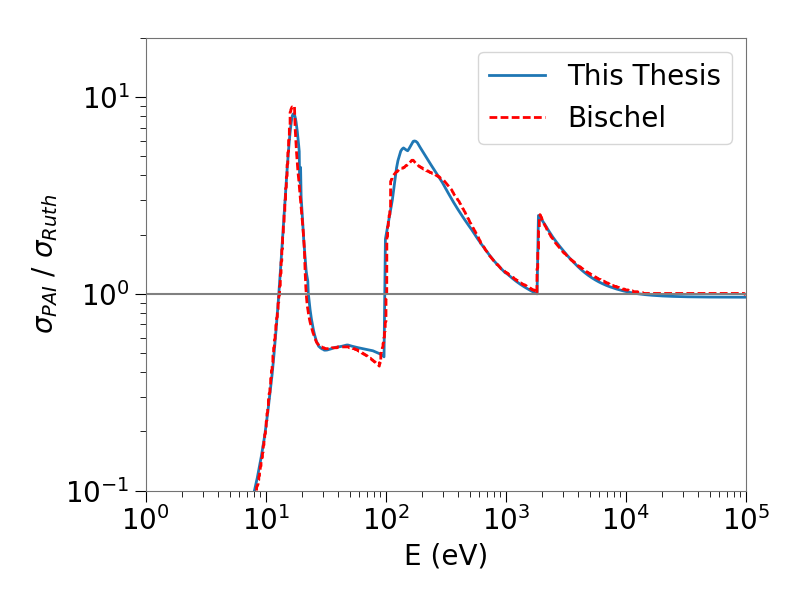
\includegraphics[width=\halffig]{figures/lips/pai_si.png}
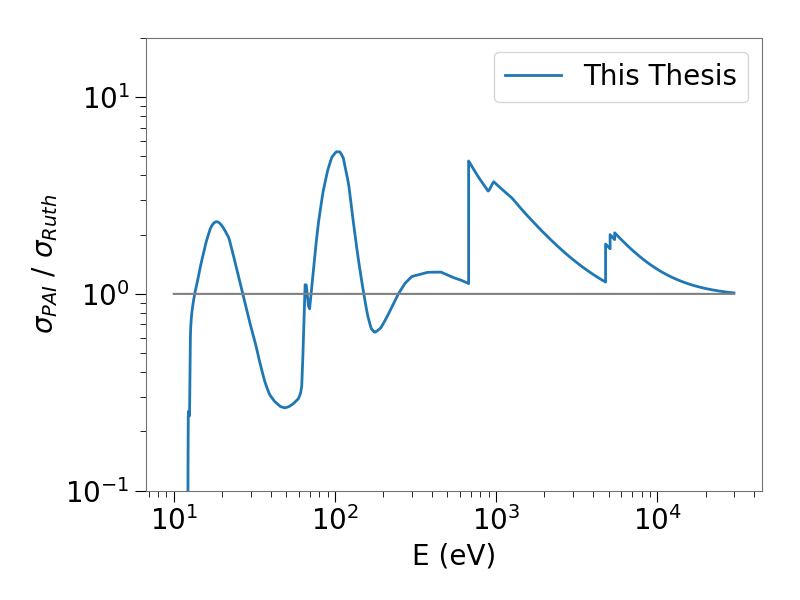
\includegraphics[width=\halffig]{figures/lips/pai_xe.png}
\caption{(left) Plot showing the deviations of the \acs{PAI} cross section from the Rutherford cross section for Si. Deviations occur at energies corresponding the M,L, and K electron shells. The result for Si is compared to \cite{Bichsel:2006} to check for agreement. (right) \acs{PAI} cross section compared to the Rutherford cross section for xenon. In both plots, the y-axes are labeled with $\sigma$ as a short-hand for $d\sigma/dE$.}
\label{fig:sigma_pai}
\end{center}
\end{figure}

To account for fractionally charged \ac{LIP}s, the only addition is a factor of $(1/f)^{2}$:

\begin{equation}
\frac{d\sigma_{PAI}(E; \beta)}{dE} \longrightarrow \Big(\frac{1}{f}\Big)^{2} \frac{d\sigma_{PAI}(E; \beta)}{dE}
\end{equation}
This cross section represents the energy transfer $E$ to an electron in a single collision. To get the total energy deposition in some thickness of absorber, we use the Monte Carlo method described in the following section.

\subsection{Straggling Monte Carlo for Energy Deposition}
In most particle physics courses, the Bethe-Bloch equation, which describes the mean rate of energy loss in materials is studied. The $\langle - dE/dx \rangle$ provided by the Bethe-Bloch equation is \textit{not} the appropriate measure for \ac{LIP} energy loss. Quoting from \cite{PDG}:

\begin{quote}
Few concepts in high-energy physics are as misused as $\langle dE/dx \rangle$. The main problem is that the mean is weighted by very rare events with large single-collision energy deposits. Even with samples of hundreds of events a dependable value for the mean energy loss cannot be obtained. Far better and more easily measured is the most probable energy loss.... The most probable energy loss in a detector is considerably below the mean given by the Bethe equation.
\end{quote}

This fact is particularly important for rare event detection: events are more likely to deposit energy near the peak of the \ac{PDF} and not the tail, where the mean energy is skewed. The probability distribution function $f(\Delta)$ that describes the energy deposited ($\Delta$) in a medium is referred to as the straggling function. Sometimes $f(\Delta)$ is referred to as a Landau function, but it is important to note that a Landau distribution does not always accurately describe straggling. In general, $f$ depends on the energy of the particle $\beta \gamma$, and the thickness of the target $X$. That is,  $f = f(\Delta; \beta \gamma, X)$. See Figure~\ref{fig:straggling} for an example of a straggling \ac{PDF} and how it can differ from the Landau distribution.

\begin{figure}[htbp]
\begin{center}
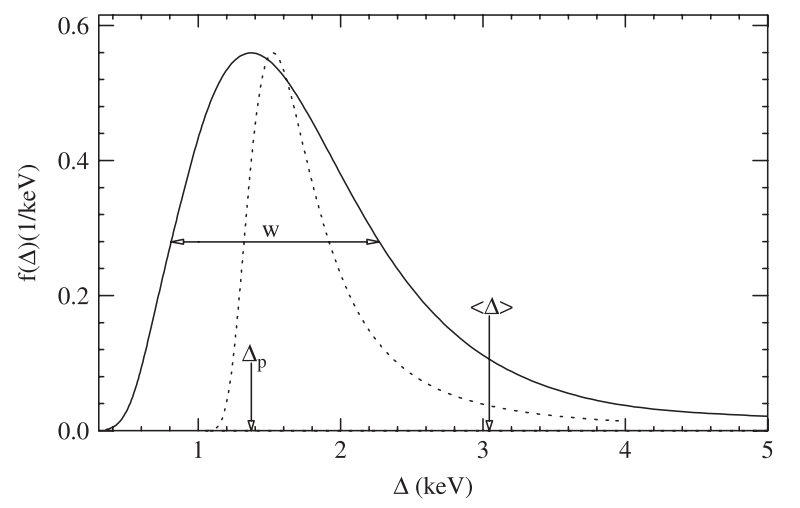
\includegraphics[width=0.8\textwidth]{figures/lips/straggling.png}
\caption{Solid line is the ``true'' straggling for particles of $\beta \gamma = 3.6$ traversing 1.2~cm of Ar gas. $\Delta_{p}$ denotes the most probable energy deposition, and $\langle \Delta \rangle$ is the average energy deposition. Note that the average energy deposition is skewed to the high tail. The dotted line shows the Landau function approximation to straggling, which is offset from the true straggling. The physical origin of the high energy tail are the rare, ``hard'' scatters with electrons. Figure from \cite{Bichsel:2006}. }
\label{fig:straggling}
\end{center}
\end{figure}

Reference \cite{Bichsel:2006} describes several methods for computing straggling functions. For this thesis the Monte Carlo method as described in \cite{Bichsel:2006} is employed. The \ac{PAI} cross section (Equation~\ref{eq:pai}) is used to calculate two quantities: $\Sigma_{t}(\beta \gamma)$, the total (macroscopic) collisional cross section, and $\Phi(E; \beta \gamma)$, the integrated single collision spectrum. These two quantities are useful because they lead to the physical quantities of mean free path, and energy lost in each collision, respectively. The following equations summarize the relationships. The total collisional cross section and its relationship to mean free path is:

\begin{equation}
\begin{split}
\Sigma_{t}(\beta \gamma) &\equiv N \int \sigma(E; \beta \gamma) dE ;\\
\lambda &\equiv 1 / \Sigma_{t}
\end{split}
\end{equation}
where $N$ is the number of atoms per cm$^{3}$, $\sigma(E; \beta \gamma)$ is the \ac{PAI} cross section as in Equation~\ref{eq:pai} (the derivate notation is dropped for simplicity), and $\lambda$ is the mean free path. The integrated single collision spectrum and its relationship to energy loss is:

\begin{equation}
\begin{split}
\Phi(E; \beta \gamma) &= \int_{0}^{E} \sigma(E^{\prime}; \beta \gamma) dE^{\prime} \big / \int_{0}^{\infty} \sigma(E^{\prime}; \beta \gamma) dE^{\prime} ;\\
E_{loss}(r)  &= \Phi^{-1}(E; \beta \gamma) 
\end{split}
\end{equation}
$\Phi(E; \beta \gamma)$, the integrated single collision spectrum, is by definition the \ac{CDF} of the energy loss for single collisions. $E_{loss}$ refers to the energy loss of a single collision. A common method used in Monte Carlo to draw a random value from a specific \ac{PDF} is to calculate the \ac{CDF} and then invert it. As for all \ac{CDF}s, the values of $\Phi$ range from [0,1]. When $\Phi$ is inverted, the resulting function $\Phi^{-1}(E; \beta \gamma)$ is defined over the range [0,1], and the dependent variable becomes $E_{loss}$. Drawing a number $r$ from a uniform random distribution between [0,1] and taking the associated y-value from an inverted \ac{CDF} results in a the original \ac{PDF} distribution. For unbiased sampling, the x-axis must be equally spaced. See Figure~\ref{fig:phi} for an illustration.

\begin{figure}[htbp]
\begin{center}
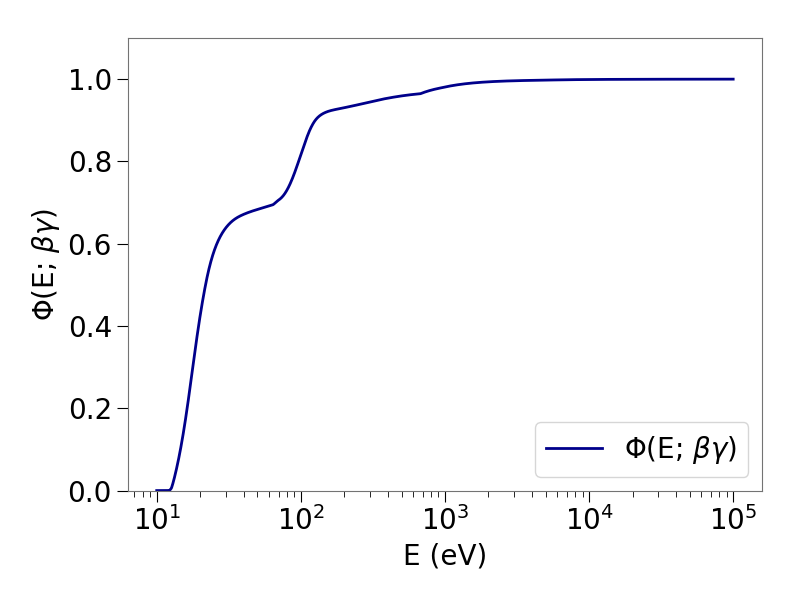
\includegraphics[width=\halffig]{figures/lips/phi.png}
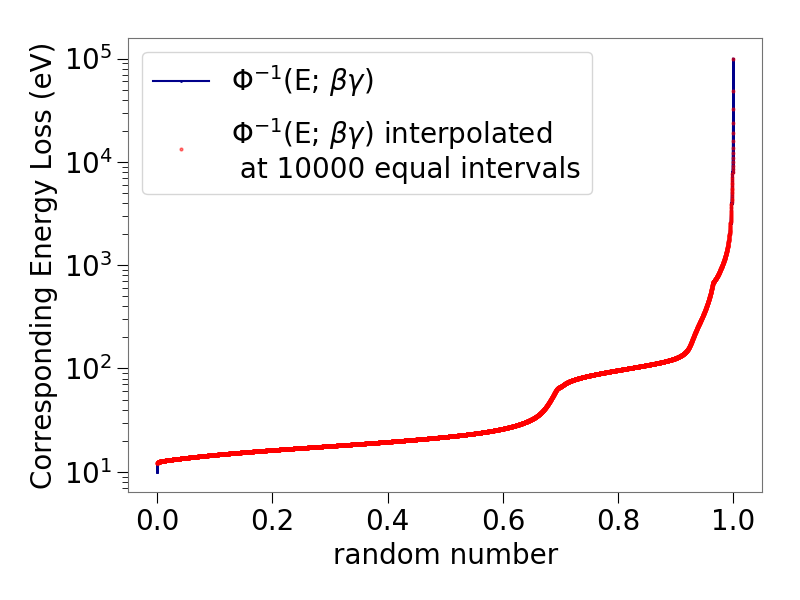
\includegraphics[width=\halffig]{figures/lips/phi_inverted.png}
\caption{(left) Plot showing $\Phi(E; \beta \gamma)$, the integrated single collision spectrum for xenon. (right) Plot showing the inverted integrated single collision spectrum for xenon, $\Phi^{-1}(E; \beta \gamma)$. In order to assure unbiased sampling of the distribution, the x-axis must be equally spaced. This can be accomplished by interpolating $\Phi^{-1}$ over an x-axis of equally spaced points from $[0,1)$. Interpolating with e.g. 10 points will result in a coarse sampling of the \acs{PDF} and interpolating with e.g. 10000 points will result in a smooth sampling. Drawing a random number $r$ gives the associated $E_{loss}(r)$. }
\label{fig:phi}
\end{center}
\end{figure}

After obtaining $\lambda$ and $E_{loss}(r)$, the Monte Carlo for a single particle traveling through a segment length $X$ and depositing energy $\Delta$ is carried out as follows:

\begin{enumerate}
\item Get the distance travelled in step $i$, $dx_{i}$. Accomplish this by drawing a uniform random number $s$, define $dx_{i} = -\mathrm{log}(s) \lambda$.
\item Get the energy deposited in step $i$, $dE_{i}$. Accomplish this by drawing a uniform random number $r$, find $dE_{i} = E_{loss}(r)$.
\item Update the total distance travelled after step $i$: $x += dx_{i}$
\item Update the total energy deposition after step $i$: $\Delta += dE_{i}$
\item If the total distance travelled $x$ is greater than or equal to $X$, exit.
\end{enumerate}

The output of the Monte Carlo can be thought of as a a collection of $dx_{i}$ and $dE_{i}$ (Figure~\ref{fig:dedx_diagram}). The result of this straggling Monte Carlo is referred to herein as the ``base'' Monte Carlo or ``1D'' Monte Carlo. 

 \begin{figure}[htbp]
\begin{center}

\includegraphics[width=\textwidth]{figures/lips/dedx_diagram.png}
\caption{A diagrammatic representation of the output of the Monte Carlo. The output for for one event is a collection of $dE_{i}$ (blue circles) and the space between them $dx_{i}$. The Monte Carlo is run many times, resulting in an accumulation of segments like these. Results of this type are referred to as the ``base 1D'' Monte Carlo. }
\label{fig:dedx_diagram}
\end{center}
\end{figure}


Repeating this procedure for many particles and histogramming the resulting $\Delta$s gives the straggling $f(\Delta; \beta \gamma, X)$ in segment length $X$. The $\beta \gamma$ energy dependence of the straggling is accounted for in the original \ac{PAI} cross section calculation (Equation~\ref{eq:pai}). The analysis assumes all \ac{LIP}s are minimum ionizing. That is, they have the energy to impart the least possible amount of energy to the medium, which occurs at $\beta \gamma \approx 4$. An example showing the results of this Monte Carlo method for a few different \ac{LIP} charge fractions is shown in Figure~\ref{fig:lip_straggling_examples}.
 
 \begin{figure}[htbp]
\begin{center}
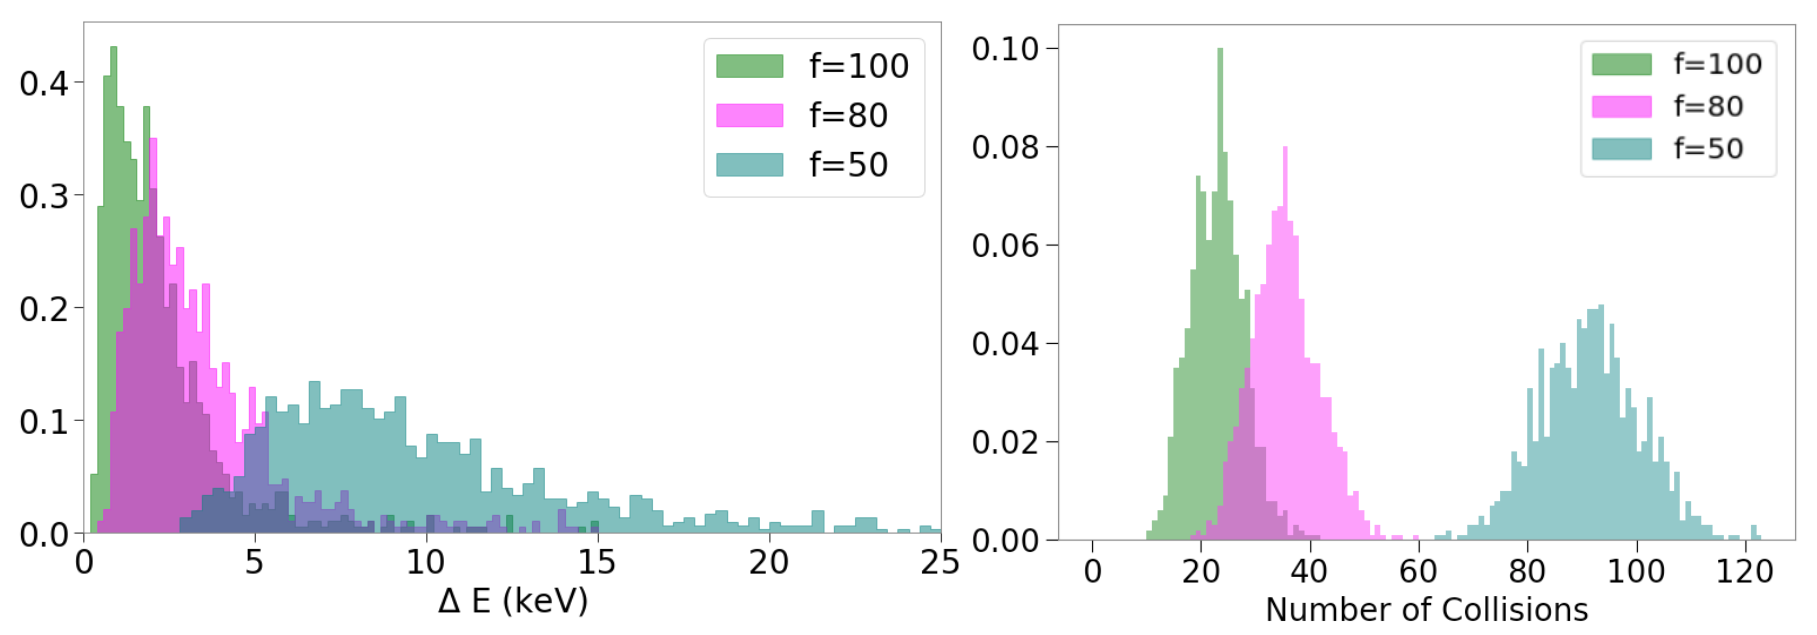
\includegraphics[width=\textwidth]{figures/lips/straggling_xe_examples.png}
\caption{(left) Plot showing the straggling for different charge fractions $f$ in 10~cm of \acs{LXe}. To generate these straggling \acs{PDF}s, the Monte Carlo described above was carried out 1000 times. (right) Plot showing the number of collisions for each charge fraction $f$.  }
\label{fig:lip_straggling_examples}
\end{center}
\end{figure}

A summary of all combinations of $f$ and path length can be seen in Figure~\ref{fig:straggling_summary}. It is useful to note that $\Phi^{-1}(E; \beta \gamma)$ is the same for all charge fractions, but $\lambda$ is a function of $f$. For high $f$, $\lambda$ is large and there are few interactions. For low $f$, $\lambda$ is small and there are many interactions. At each interaction, the same distribution of energies is sampled but for low $f$ there are far more interactions and therefore more energy deposition total. 


 \begin{figure}[htbp]
\begin{center}
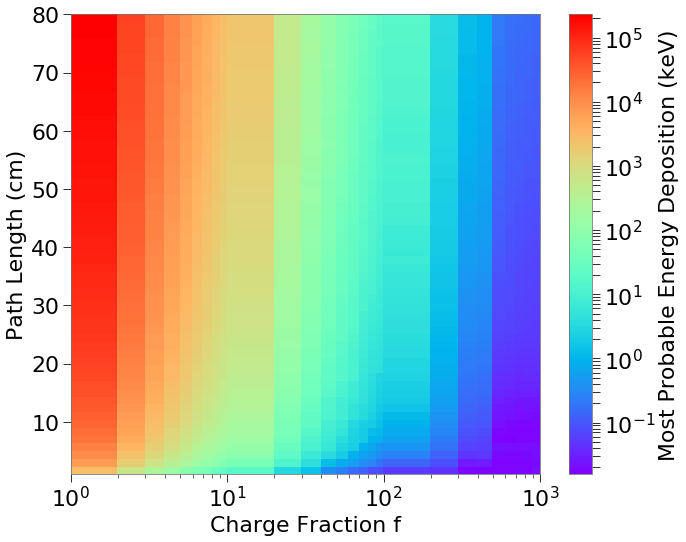
\includegraphics[width=\halffig]{figures/lips/dEprob.png}
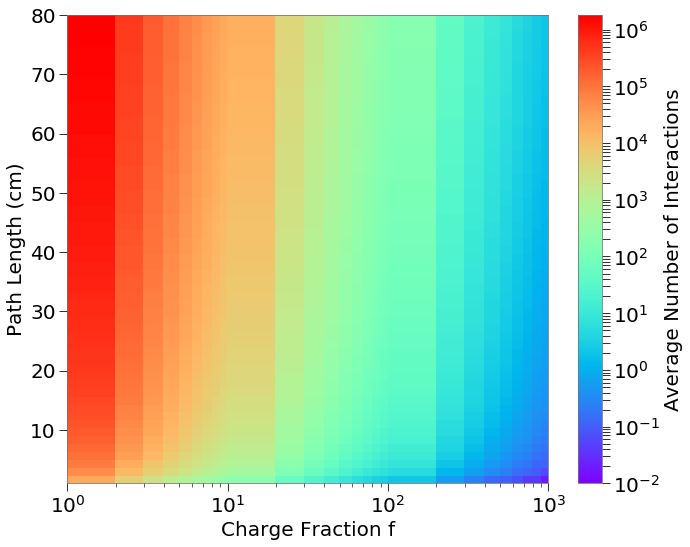
\includegraphics[width=\halffig]{figures/lips/avg_hits.png}
\caption{(left) The most probable energy deposition for a given charge fraction traveling though a path length of \acs{LXe}. The plot was generated by carrying out the Monte Carlo described above, histogramming the results, and finding the peak of the distribution. (right) The average number of interactions for a \acs{LIP} of charge fraction $f$ traveling though a path length of \acs{LXe}. }
\label{fig:straggling_summary}
\end{center}
\end{figure}

To better illustrate the stochastic nature of straggling, the energy deposition per unit length for different path lengths was found for each charge fraction (see Figure~\ref{fig:stochastic}). For higher $f$, there are fewer expected depositions total and so one may expect a lower value for energy deposition per unit length in, say, 10.0~cm than 80.0~cm, but that is not what happens. While most events of $f=1000$ won't interact at all in 10.0~cm of \ac{LXe}, there are a few, rare events that bias the result. The effect of these rare events is washed out over a longer path length of 80.0~cm. This is why an 80.0~cm ``measure'' of $dE/dx$ results in a lower value than a 10.0~cm measure. Since low $f$ have many millions of interactions in a few centimeters, the effect of a few additional interactions will not change the result very much. Therefore, the stochastic straggling is less visible for low $f$. To validate the accuracy of this Monte Carlo method, the average energy deposition for \ac{LIP}s of different $f$ is compared to $\langle dE/dx \rangle_{0} f^{-2}$, where $\langle dE/dx \rangle_{0}$ represents the average energy loss per unit length for a muon at minimum ionization from reference \cite{PDG}. As expected, \ac{LIP} energy depositions also fall off as $f^{-2}$, but the \ac{LIP} values were found to be 13\% lower than the value stated in \cite{PDG}. This offset is treated as a systematic uncertainty, see Section~\ref{sec:systematics} below.

 \begin{figure}[htbp]
\begin{center}
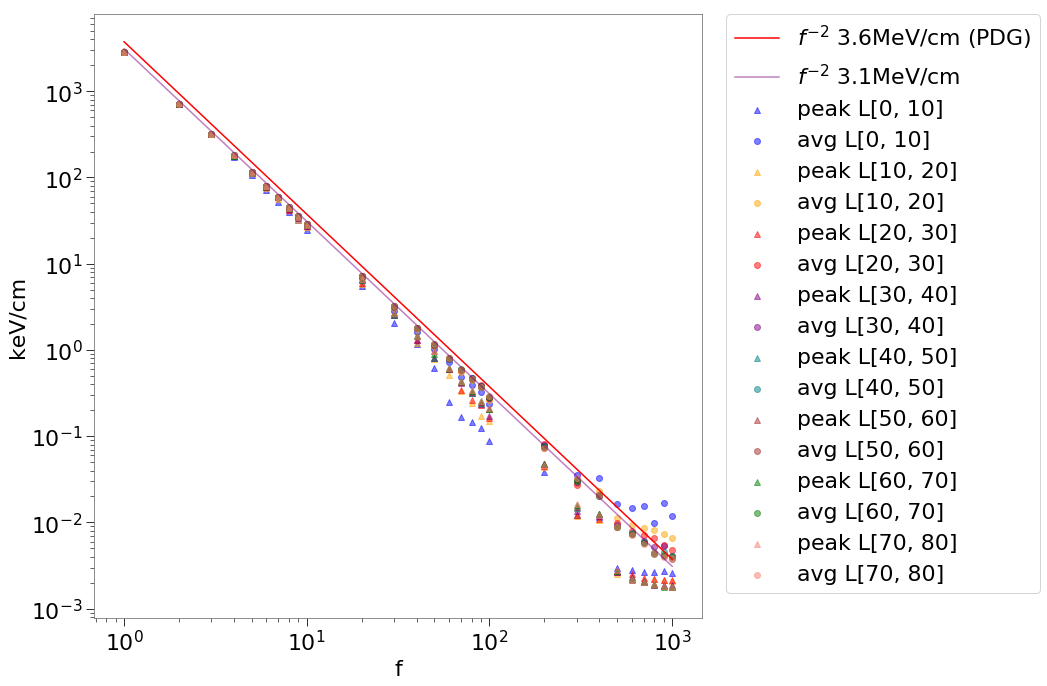
\includegraphics[width=\textwidth]{figures/lips/stochastic_wPDG.png}
\caption{Plot showing the peak (triangle) and the average (circle) of energy deposition in different path lengths. At high charge fraction, interactions are less likely, and so are greatly affected by statistical deviations. The line is $f^{-2}$3.1~MeV/cm, as energy deposition for \acs{LIP}s falls off as $f^{-2}$. The value expected at $f=1$ ($\langle dE/dx \rangle$ for a muon) is 3.6~MeV/cm \cite{PDG} (red line); our result is 13\% lower than this. Reference \cite{PDG} gives the energy loss in units of MeV~g$^{-1}$~cm$^{2}$, a \ac{LXe} density of 2.94~g/cm$^{3}$ is used to translate to MeV/cm. This is the same value for \acs{LXe} density used in the straggling Monte Carlo.  }
\label{fig:stochastic}
\end{center}
\end{figure}

 
\subsection{Downsampling for 3D Distribution}
This section describes how a 1D Monte Carlo segment as in Figure~\ref{fig:dedx_diagram} is used to generate 3D events in the \ac{LUX} geometry; the scheme is represented in Figure~\ref{fig:downsample}. The incoming \ac{LIP} distribution is assumed to be isotropic from above. In order to simulate this, a generator was written for LUXSim, the \ac{LUX} Collaboration's Geant4-based simulation. More details can be found about LUXSim in \cite{LUXSim}. The generator created primary particles on a hemisphere centered at $(0,0,h)$ where $h$ refers to the height of the \ac{LUX} detector in the LUXSim geometry. The particle positions were uniform random on the hemisphere and the particle momenta were a uniform random direction on the unit sphere. Such an initial distribution will result in the majority of particles not entering the \ac{LUX} detector, so a downsampling method was used. Instead of simulating \ac{LIP}s with this hemispherical generator, geantinos were used. Geantinos are artificial, non-interacting particles from Geant4 that only generate a step action when crossing geometry boundaries. If a geantino was observed to enter the \ac{LXe} volume of the detector, its initial position, momentum, and \ac{LXe} entrance and exit positions were saved to a file. Drawing from this file provided an initial position and momentum (direction) for a \ac{LIP} to enter the \ac{LXe} volume of the \ac{LUX} detector. The \ac{LIP} was then propagated according to its base 1D Monte Carlo until it left the \ac{LXe} volume (see Figure~\ref{fig:downsample}).


\begin{figure}[htbp]
\begin{center}
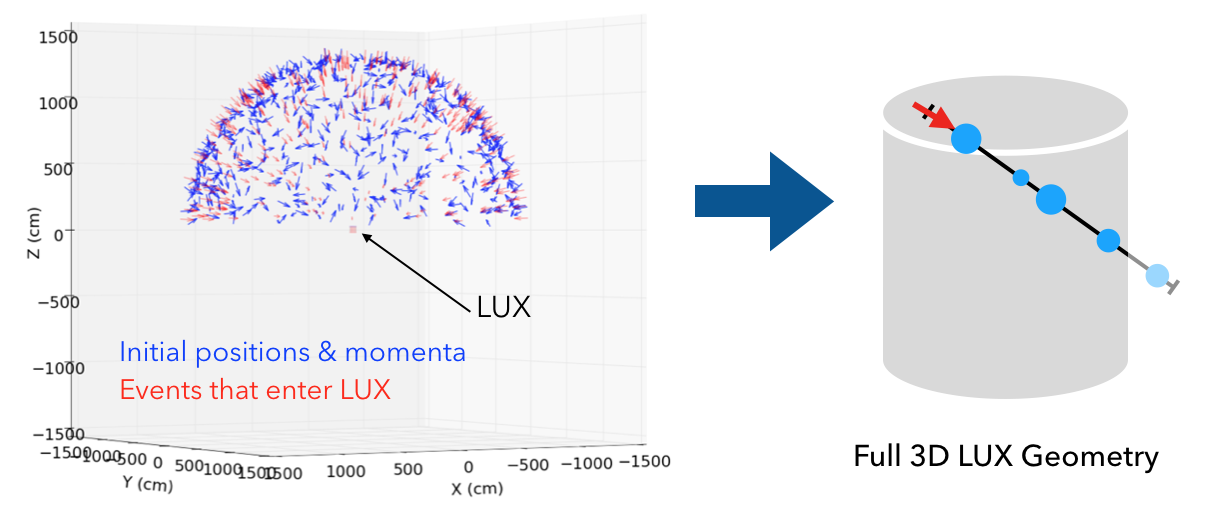
\includegraphics[width=\textwidth]{figures/lips/downsample.png}
\caption{Diagram illustrating the downsampling method for \acs{LIP}s. Geantinos were generated with uniform random position and momentum on a hemisphere. If a geantino entered the \acs{LXe} volume of the detector, the position where it entered the \acs{LXe} was saved along with its momentum. The base 1D Monte Carlo was then ``injected''  into the \acs{LXe} with this position and momentum and propagated until it left the \acs{LXe} volume. }
\label{fig:downsample}
\end{center}
\end{figure}

\subsubsection{Solid Angle Calculation}
The solid angle $\Omega$ was calculated from the geantino simulation output. As described above, the positions and momenta of the events that entered the \ac{LXe} space of the \ac{LUX} detector were saved. The initial positions of these events were histogrammed, as in Figure~\ref{fig:skymap}. The acceptance for events coming from near vertical polar angles is small, because only a few initial momenta will allow the particle to enter \ac{LUX}. For large polar angles, the acceptance grows because many initial momenta will result in success. 

\begin{figure}[htbp]
\begin{center}
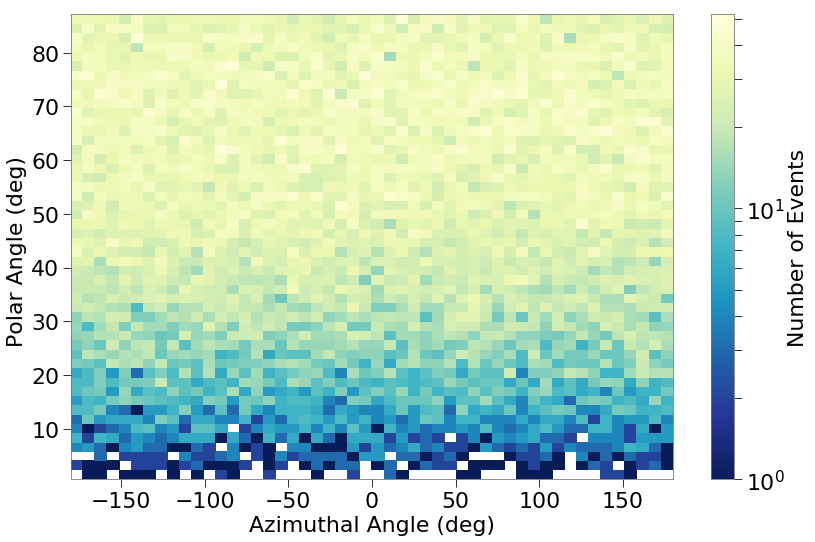
\includegraphics[width=\textwidth]{figures/lips/skymap.png}
\caption{A 2D histogram of the initial positions for geantinos that entered the xenon space of \acs{LUX}. Polar angle indicates deviation from the vertical. }
\label{fig:skymap}
\end{center}
\end{figure}

Since the map of initial positions in the $(\theta, \phi)$ plane is azimuthally symmetric, the $\theta$-projection was taken, counts were normalized to one, and bin density was normalized to $2\pi$~str. Then the integral was taken to give the solid angle. This procedure was done for several different bin sizes (26 trails of integer bins from 25 $\times$ 25 bins up to 50 $\times$ 50 bins) and the average was taken to reduce the effect of binning. The result is $\Omega_{LUX} = 3.78 \pm 0.04$, where the error is the standard deviation of the results for the different bin sizes. The effect of normalizing to $4\pi$~str was tested, and it did not change the results. 

\subsection{Generating PMT Waveforms}
This section describes how the 3D straggling Monte Carlo is used to generate \ac{PMT} waveforms, so the full \ac{LUX} detector response can be assessed. Recall that an energy deposition in \ac{LXe} produces scintillation photons and ionization electrons. One method is to generate the photons as secondary particles and do a full optical simulation following their paths until they end in a \ac{PMT} and generate a photoelectron. The electrons would be drifted under the influence of the electric field, extracted into the gas region, where they would then generate more photons from their proportional scintillation in the gas, and these photons would be similarly propagated through the detector until they end in a \ac{PMT} and generate a photoelectron. This method, with full tracking and optical simulation of the secondaries, is prohibitively slow and computationally intensive for \ac{LIP}s, which can have $O(100)$ primary interactions in the detector. 

The method used for generating photoelectrons in the \ac{PMT}s was a \ac{LUX} Collaboration internal piece of software called fastSim. Instead of calculating the trajectory and reflection(s) of every photon, fastSim uses the position and numbers of initial quanta to ``directly transport'' photons to their statistically-determined final destinations. The number of initial quanta (scintillation photons and ionization electrons) are determined by G4S1Light.cc, which includes a clustering of any energy depositions within 0.04~cm of each other. This merges nearby hits of energies $E_{1}$ and $E_{2}$ to a single hit of $E = E_{1} + E_{2}$, with the requisite number of quanta. The choice of clustering radius is based on \cite{Mozumder1995}, and is related to how far electrons travel before thermalizing. The resulting output is an \textbf{.evt}-file which contains \ac{PMT} waveforms of \ac{LIP} events (see Chapter~\ref{sec:lux_dpf} for details about \textbf{.evt}-files). An example of an $f=100$ \ac{LIP} is shown in Figure~\ref{fig:visualux_f100}.

\begin{figure}[htbp]
\begin{center}
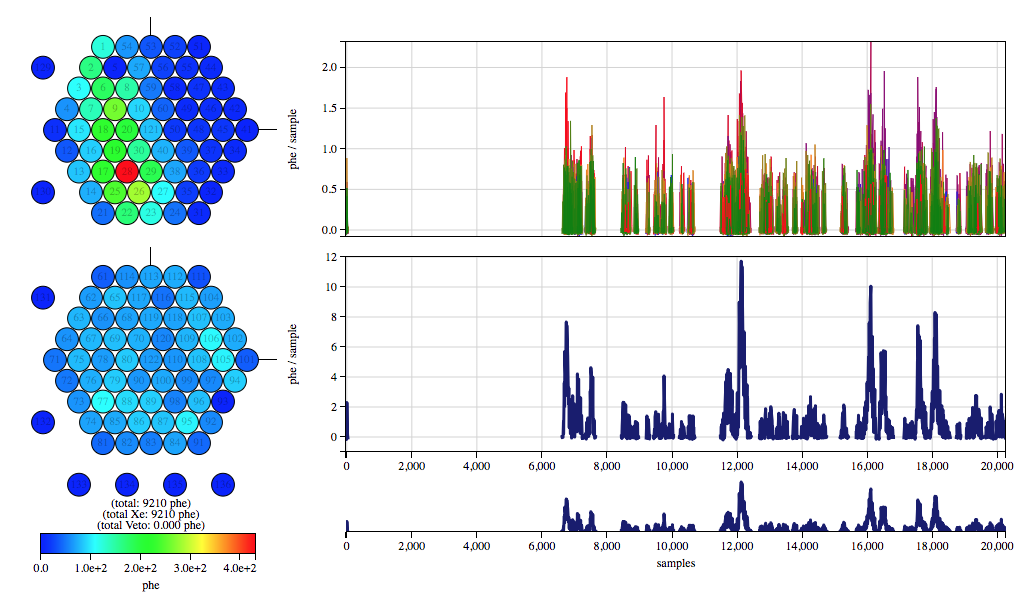
\includegraphics[width=\textwidth]{figures/lips/visualux_f100.png}
\caption{The simulated detector response to a \acs{LIP} of charge fraction $f=100$. The hexagonal maps filled with circles represent the top and bottom \acs{PMT} arrays. The color scale indicates how many photons were observed in each \acs{PMT}. The top graph shows each \acs{PMT} voltage trace in a different color, and the bottom graph shows the summed \acs{PMT} waveforms.  }
\label{fig:visualux_f100}
\end{center}
\end{figure}

\FloatBarrier
\subsection{PMT Waveform Processing}
The \ac{PMT} waveforms were processed with the default \ac{LUX} \ac{DPF}, except that the number of pulses was increased from 10 to 100. That is, up to 100 pulses could be found in an event. No changes were made to the pulse finder or the definitions of the five types of pulses: S1, S2, SE, SPHE, and Else. The \ac{LUX} data processing was intended for use on single-scatter events with only one S1 and one S2. Thus, its performance for \ac{LIP} events, which have many pulses, is not expected to be ideal. An example of the \ac{DPF} run on an $f=100$ event is shown in Figure~\ref{fig:visualux_f100_dp}. This is the same event shown above in Figure~\ref{fig:visualux_f100}. Visible in the data processing are examples of two S2s being merged into one (pink dotted lines). Issues like these have repercussions for the position reconstruction and energy reconstruction. 

\begin{figure}[htbp]
\begin{center}
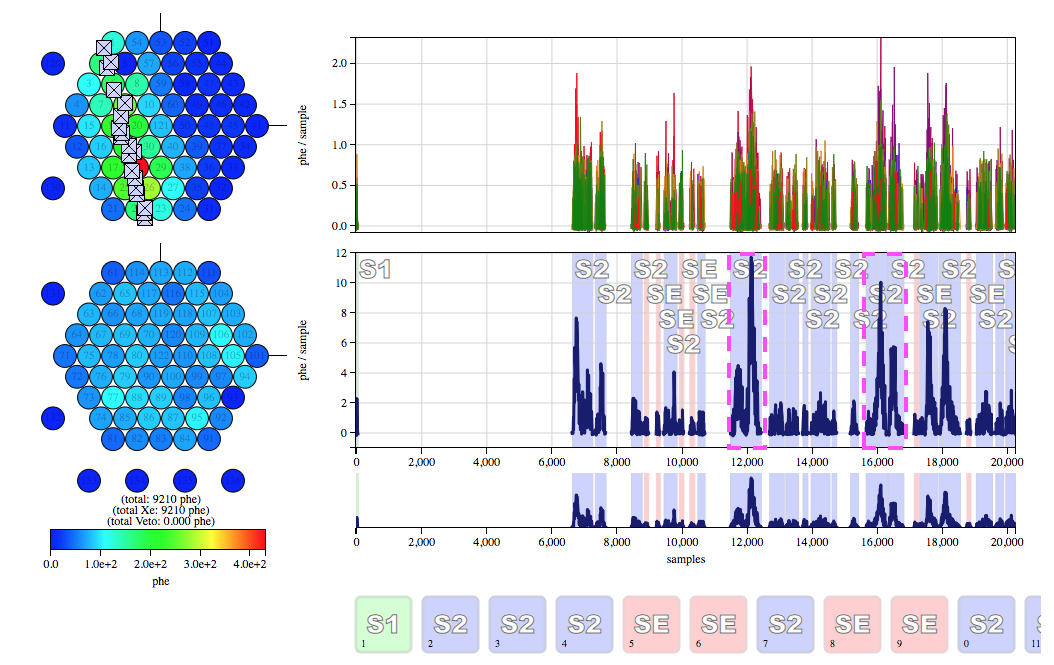
\includegraphics[width=\textwidth]{figures/lips/visualux_f100_dp.png}
\caption{The result of the \acs{LUX} \acs{DPF} on a \acs{LIP} of charge fraction $f=100$. The pink dashed lines highlight energy depositions that were merged by the pulse finder. The ``x'' markers on the \acs{PMT} map indicate the Mercury reconstructed positions, which have position corrections applied. }
\label{fig:visualux_f100_dp}
\end{center}
\end{figure}
%luxsm_20180621T0100 event 10

The data processing plays a large role in the \ac{LIP} analysis. A few merged pulses like those in Figure~\ref{fig:visualux_f100_dp} do not greatly limit the capability to do track reconstruction, but with lower $f$, where more energy is deposited, the pulse finder effects are magnified. Two examples of an $f=10$ \ac{LIP} with the \ac{DPF} results are shown in Figure~\ref{fig:visualux_f10_dp} and Figure~\ref{fig:visualux_f10_dp_2}. 

\begin{figure}[htbp]
\begin{center}
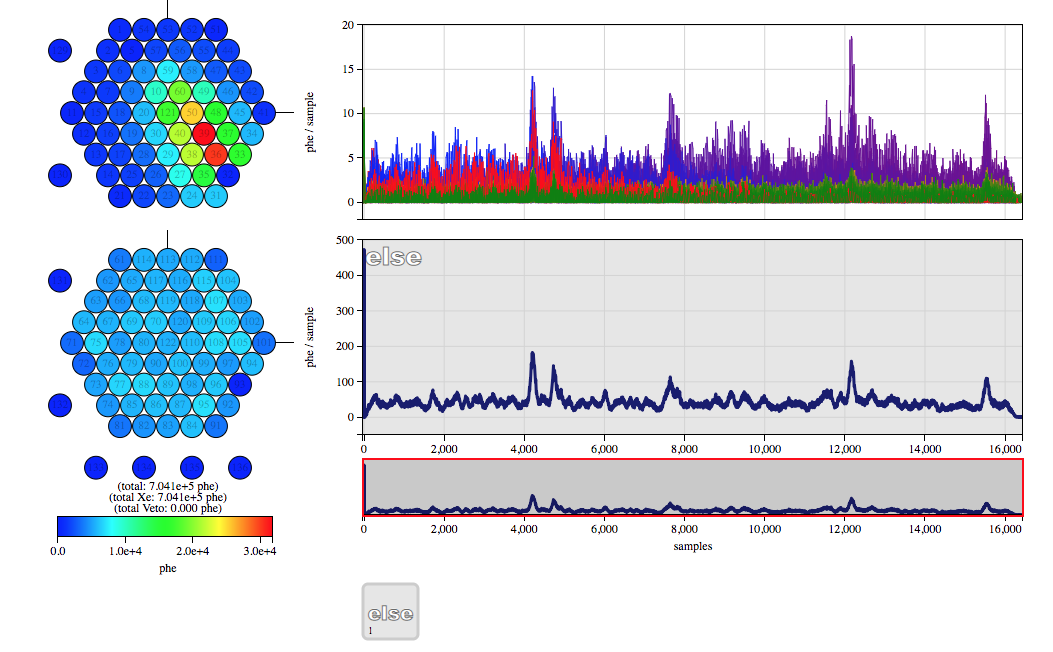
\includegraphics[width=\textwidth]{figures/lips/visualux_f10_dp.png}
\caption{The result of the \acs{LUX} \acs{DPF} on a \acs{LIP} of charge fraction $f=10$. The pulse finding capability was seen to fall dramatically with decreasing $f$. This event traversed the detector starting near \acs{PMT}s 53 and 52, and proceeded across to \acs{PMT}s 23 and 24.}
\label{fig:visualux_f10_dp}
\end{center}
\end{figure}
%luxsm_20180621T0010 one of first 10 events

The pulse finder often failed to isolate individual pulses for low $f$ and the entire event would be classified as an Else pulse (Figure~\ref{fig:visualux_f10_dp}). Sometimes, the pulse finder successfully broke the ionization trail into successive S2 and/or Else pulses (Figure~\ref{fig:visualux_f10_dp_2}). However, these pulses often failed the Mercury position reconstruction and correction algorithms. These types of pulse finder effects have consequences especially for track reconstruction and they decrease the detection efficiency for \ac{LIP}s for low $f$. This turnover in efficiency for low $f$ is somewhat counter-intuitive: typically we think of detection efficiency in \ac{LXe} \ac{TPC}s as a function of energy deposition; if the energy deposition is large enough, we see a signal. Low $f$ \ac{LIP}s certainly deposit enough energy to produce a signal, but ability to reconstruct a track is a major factor in the detection efficiency for \ac{LIP}s. It was found that the efficiency for finding corrected S2 pulses dropped off sharply below $f=10$; therefore, this analysis employs an $f=10$ cut off, and does not carry out a search for any lower charge fractions. 

\begin{figure}[htbp]
\begin{center}
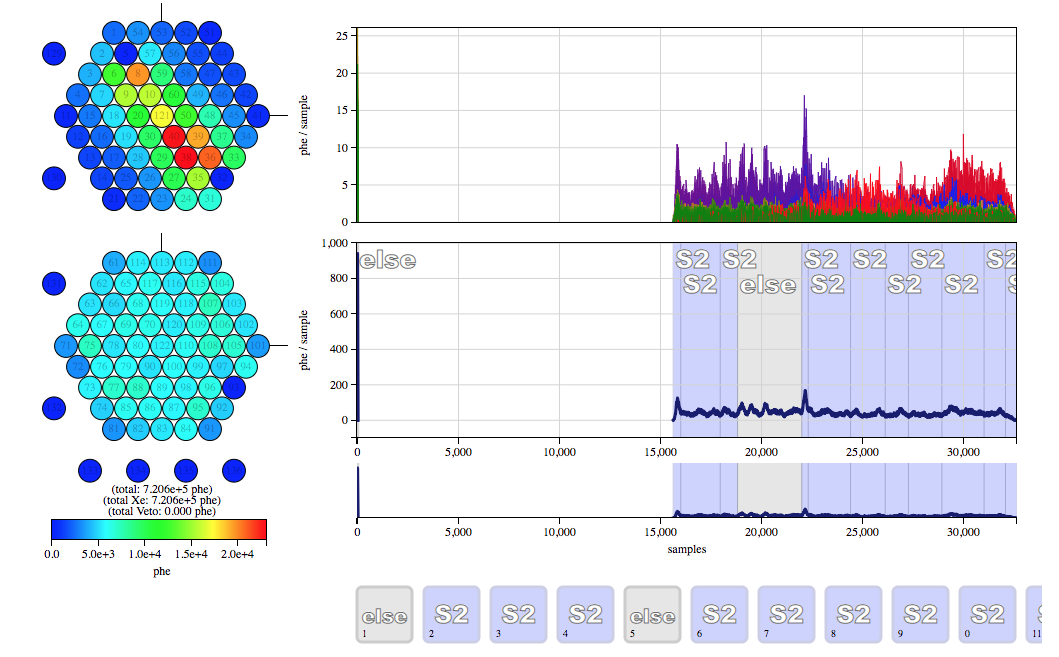
\includegraphics[width=\textwidth]{figures/lips/visualux_f10_dp_2.png}
\caption{The result of the \acs{LUX} \acs{DPF} on a \acs{LIP} of charge fraction $f=10$. The pulse finding capability was seen to fall dramatically with decreasing $f$. The pulse finder was sometimes able to isolate individual S2s for low $f$ events, but the Mercury reconstruction of these events often failed. There are no positions marked on the \acs{PMT} hit map for this event, indicating that position reconstruction failed.   }
\label{fig:visualux_f10_dp_2}
\end{center}
\end{figure}
%luxsm_20180621T0010 one of first 10 events

The energy reconstruction is also affected by the pulse finder identifying area as Else instead of S2. Figure~\ref{fig:dEdx_reconstructed} contains the reconstructed energy deposition for charge fractions in the range $f = [10,1000]$. The energy is reconstructed the usual way: $E = W (S1/g1 + S2/g2)$ and the per-event track length $L$ reconstruction is discussed further below in Section~\ref{sec:lip_filter}. The factor $E/L$ was reconstructed for several events and charge fractions, and the results were histogrammed. Plotted is the average of such histograms for each charge fraction $f$. For low $f$, the corrected energy is systematically lower due to the pulse finder. Only corrected S2 area is used in the reconstruction, so any area going into Else pulses is ``lost''. At high $f$, the result for reconstructed $dE/dx$ is higher than the expected trend line due to the bias discussed earlier: for high $f$, only very few high-energy events are above threshold, which biases the measure to the high energy tail. Compare Figure~\ref{fig:dEdx_reconstructed} to Figure~\ref{fig:stochastic}.

\begin{figure}[htbp]
\begin{center}
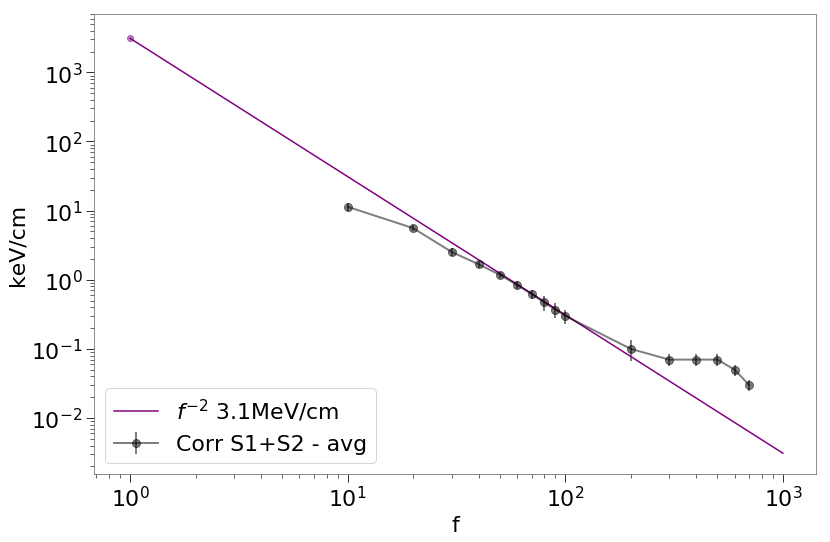
\includegraphics[width=\textwidth]{figures/lips/dEdx_reconstructed.png}
\caption{The reconstructed $dE/dx$ for several charge fractions. The plot was generated by reconstructing the energies $E$ and track lengths $L$ from \acs{LIP} waveforms that were processed with the \acs{LUX} \acs{DPF}. The $E/L$ from each event was added to a histogram, and the averages of the histograms for each simulated $f$ were found. The detector response matches expectations from the \acs{PAI} cross section in the charge range $f = [50, 200]$ (compare to Figure~\ref{fig:stochastic}). Below this range, the pulse finder yields a ``loss'' of any non-S2 area. Above the range, only the highest energy fluctuations are detected; and the detector response levels off due to low statistics (most events are in the first bin, but there are many events which did not deposit enough energy to be ``measured'', i.e. to make it into the histogram). }
\label{fig:dEdx_reconstructed}
\end{center}
\end{figure}



\FloatBarrier
\section{LIP Filter}
\label{sec:lip_filter}
After the waveform data is processed into \ac{RQ} files, there is another step of processing referred to as the Filter Code. For the \ac{WIMP} analysis, all multi-scatter events are rejected. So-called \ac{WIMP} ``golden events'' with one S1 and one S2 are filtered from the months of live data. Once selected, the \ac{WIMP} golden events were further paired down based on reconstructed position, energy, and whether they were \ac{ER} or \ac{NR}. Thus any remaining events in the fiducial volume with an energy in the \ac{WIMP} search range below the \ac{NR} mean are \ac{WIMP} candidates. In the same vein, a \ac{LIP} Filter was developed. The \ac{LIP} Filter was designed to read in \ac{RQ} files, and \textit{keep} the multi-scatter events, as these are the potential \ac{LIP} candidates. The \ac{LIP} filter code also produces additional \ac{RQ}s that are useful in identifying a \ac{LIP}. Every new \ac{LIP} \ac{RQ} was produced three times with a different definition of ``multi-scatter''. That is, each event was filtered for (1) Corrected S2s (2) Raw S2s and (3) Raw S2-like pulses, which refers to S2, Else, and SE pulses following an S1. In each case, a \ac{LIP} \ac{RQ} was calculated. For example, one \ac{LIP} \ac{RQ} is the sum of all the S2 area. For case (1) the S2 pulses with position-corrected areas were summed (see Chapter~\ref{sec:krypton} for a description of the pulse area corrections applied with the $^{83m}$Kr calibration). For case (2) the raw S2 area (with no corrections) were summed. For case (3) the raw S2 and raw Else and raw SE area were summed. It should be noted that by default the \ac{LUX} \ac{DPF} does not apply pulse area or position corrections to Else and SE pulses. Three different pulse filters were used because at the time of the \ac{LIP} Filter development, it wasn't clear which case, (1), (2), or (3) would result in the most useful and robust \ac{RQ}s for identifying \ac{LIP} candidates. This section summarizes the \ac{RQ}s calculated by the \ac{LIP} Filter, and the following section discusses which \ac{RQ}s were ultimately used in the \ac{LIP} analysis. A list of all the \ac{RQ}s contained in the \ac{LIP} Filter output is given in Appendix~\ref{app:lipfilter}. 

\subsection{Track Reconstruction and RQs}
One of the assumptions made in the \ac{LIP} search is that \ac{LIP}s are cosmogenic and relativistic. They are expected to enter the detector isotropic in the upper 2$\pi$ and proceed through the detector without any deviation. Thus, the \ac{LIP} search requires track reconstruction. Two track reconstruction algorithms were developed, and since each event was split into 3 cases ( (1) Corrected S2, (2) Raw S2, and (3) Raw S2-like), an event could be fit up to six times. The time spent on track fitting was the most time consuming part of the \ac{LIP} filter. The first track fit minimizes the following expression:

\begin{equation}
\label{eq:chi2}
\chi^{2} = \sum_{i}^{n} \Big( \frac{d_{i}}{\sigma_{t_{i}}} \Big)^{2}
\end{equation}
where $n$ is the number of pulses for case (1), (2), or (3), as defined above, $d_{i}$ is the perpendicular distance from point $i$ to the fit line, and $\sigma_{t_{i}}$ is the ``total error'' for point $i$ from the Mercury position reconstruction. The error from position reconstruction is parametrized in this manner because by default, Mercury returns the reconstruction errors in the cylindrical coordinates, ($r, \phi$) (see \cite{LUXPositionReconstruction}). However, positions are stored and position corrections are applied in \ac{RQ} files in cartesian coordinates ($x, y$). The entire covariance matrix of the position errors is not kept, so any attempt to translate the ($r, \phi$) errors into errors on ($x, y$) would lose any underlying correlation. Therefore, the errors were added in quadrature to yield $\sigma_{t}$ for each point, which can be thought of as sphere parametrizing the error in all directions, instead of separately in the $x$ and $y$ directions. An error of 1.0~cm was applied for the $z$-direction, to help account for the fact that \ac{LIP} interactions are spread out along their tracks instead of being point-like. The $\chi^{2}$ in Equation~\ref{eq:chi2} is the minimization variable\footnote{This variable is actually more of a likelihood than a true $\chi^{2}$, since there is no reason to believe the $\sigma_{t}$ errors are gaussian. However, the \ac{LIP} filter code refers to the track minimization as $\chi^{2}$ and to avoid confusion for anyone using the \ac{LIP} filter in the future, we try to refer to variables here with the same names.}, and each iteration of the fit tries new parameters for a line in 3D (see Figure~\ref{fig:chi2_diagram}). The parameters that minimize $\chi^{2}$ define the \ac{LIP} track. 

\begin{figure}[htbp]
\begin{center}
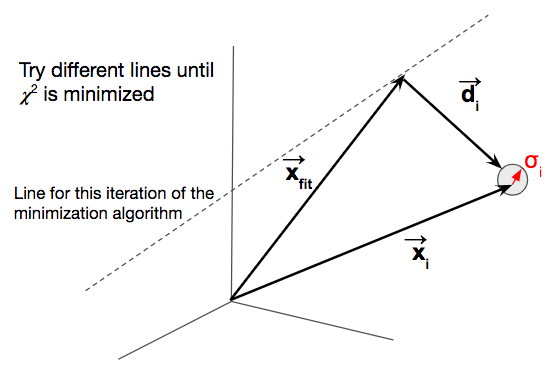
\includegraphics[width=\textwidth]{figures/lips/chi2_diagram.png}
\caption{A diagram of the $\chi^{2}$ minimization variable for track reconstruction. The figure shows the example of one point, e.g. the corrected reconstructed position of one S2 pulse. A minimum of three points was required by the \acs{LIP} Filter for track reconstruction, so that a $\chi^{2}$ may be defined.   }
\label{fig:chi2_diagram}
\end{center}
\end{figure}

Another $\chi^{2}$ is also defined in the \acs{LIP} filter, to penalize irregular deflections and spacing between the points. The minimization variable is defined as follows:

\begin{equation}
\label{eq:chi2_anglePen}
\chi_{anglePen}^{2} = \sum_{i}^{n} \Big( \frac{d_{i}}{\sigma_{t_{i}}} \Big)^{2} +\sum_{i, j=i+1}^{n-1}  \Big( \frac{\theta_{i,j} - \bar{\theta}_{i,j}}{\Delta \theta_{i,j}} \Big)^{2}+ \Big( \frac{d_{i,j} - \bar{d}_{i,j}}{\Delta d_{i,j}} \Big)^{2}
\end{equation}
where the $d_{i,j}$ is the distance between consecutive points and $\theta_{i,j}$ is the angle from dot produce between the vector $\vec{d}_{i,j}$ and the direction vector of the line. The bar notation (e.g. $\bar{\theta}_{i,j}$) represents the average of the variable and the $\Delta$ notation (e.g. $\Delta \theta_{i,j}$) represents the standard deviation of the variable.

A number of track-related \ac{LIP} \ac{RQ}s are calculated and saved to the \ac{LIP} Filter output. Both $\chi^{2}$ values described above are saved, along with the number of degrees of freedom for each event and fit. The reconstructed track length $L_{fit}$ is also saved by using the fit result to determine where the \ac{LIP} entered and exited the detector. The polar and azimuthal angles of the track, and the parameters that define the line are also saved. Another useful track \ac{RQ} was found to be the standard deviation of the distances between points. 

%It was found that the reconstructed track length was robustly returned the simulated track length, i.e. the track reconstruction method above described the distance the \ac{LIP} was propagated in LUXSim. 

Examples of track reconstruction using position corrected S2s are shown in Figure~\ref{fig:tracks_f100} for $f=100$. The colors indicate different events and the markers are scaled by S2 pulse area.

\begin{figure}[htbp]
\begin{center}
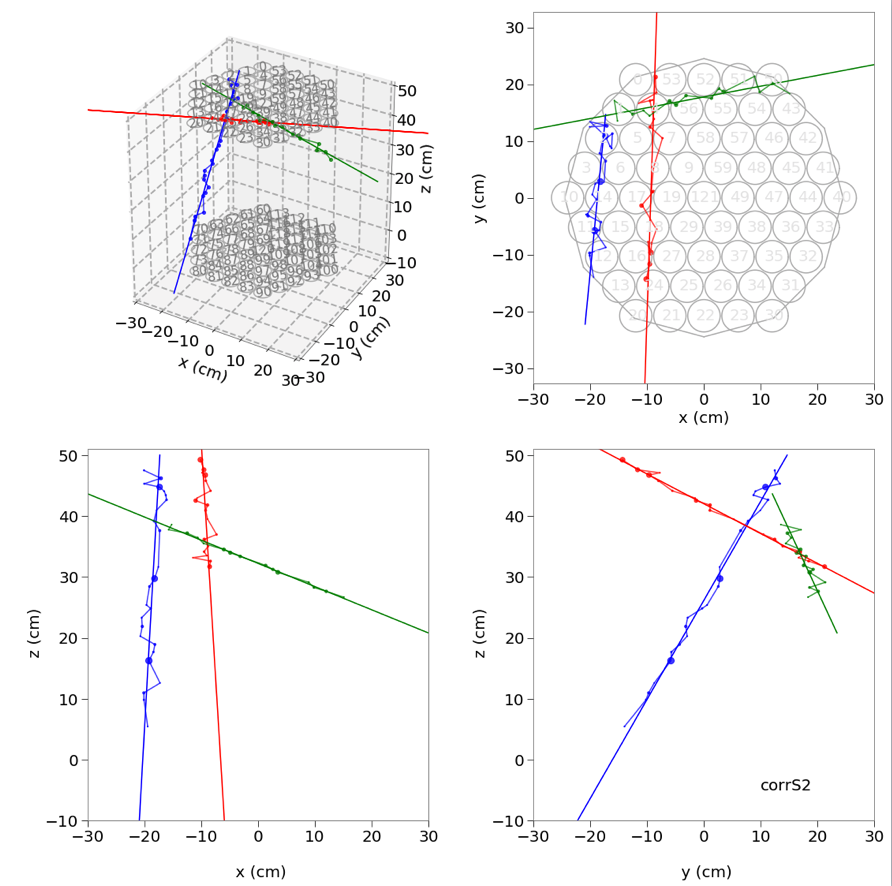
\includegraphics[width=\textwidth]{figures/lips/tracks_f100.png}
\caption{The result of track reconstruction for $f=100$ \acs{LIP}s using the $\chi^{2}$ in Equation~\ref{eq:chi2} as the minimization variable. Each color represents a different \acs{LIP} event. The panels show the full 3D view (top left), the top-down view in $(x,y)$ (top right), and two side views $(x,z)$ and $(y,z)$ (bottom left and right, respectively.) }
\label{fig:tracks_f100}
\end{center}
\end{figure}


\subsection{Energy Consistency RQs}
One of the guiding principles from the \ac{LIP} straggling discussed above is that \ac{LIP}s passing through the \ac{LUX} detector are expected to deposit their energy around some most probable value. If one divided up a \ac{LIP} track into, e.g. 10~cm segments, each segment will contain a deposition drawn from the related straggling \ac{PDF} $f(\Delta; (\beta \gamma)_{min}, X=10~\mathrm{cm})$. Most of these ``random draws'' from the straggling \ac{PDF} will be at the peak of the distribution, since the first 10~cm of \ac{LXe} are no different from the next; by assumption the \ac{LIP} does not lose enough energy to change its energy deposition behavior over the height or width of the \ac{LUX} detector. Therefore, the energy-related \ac{RQ}s are mainly developed to test whether the energy deposition along the track adheres to this expected behavior, and are not concerned with accurately measuring the total energy deposition itself. 

Some examples of useful \ac{RQ}s that test the energy consistency of events are: the standard deviation of the pulse areas and the ratio of the first two pulse areas to the last two pulse areas. Another energy consistency \ac{RQ} that was utilized was the Anderson-Darling test statistic. The Anderson-Darling test belongs to a class of test statistics that determine if a collection of observations are drawn from a given \ac{PDF}. Other such test statistics are the Kolmogorov-Smirnov and Cramer von Mises test statistics. All of these tests were tried, and it was found that the Anderson-Darling test had the best performance for rejecting background. The test is a measure of the weighted quadratic difference between the hypothetical distribution $F$ and the sample distribution $F_{n}$:

\begin{equation}
A^{2} = n \int_{-\infty}^{\infty} \frac{ (F_{n}(x) - F(x))^{2}}{F(x)(1-F(x))} dF(x)
\end{equation}
where $A$ is the Anderson-Darling test statistic. Figure~\ref{fig:energy_distribution_lip_bkg} illustrates the differences between \ac{LIP} and background straggling (the backgrounds are discussed in the following section). Each event with a reconstructed track was binned into 10 equal-sample bins\footnote{The number of bins was chosen by testing 6, 10, and 50 bins. A choice of 50 bins slowed down the calculation appreciably, and resulted in poorer background rejection. A choice of 10 bins did not take significantly more time than 6 bins, and showed better background rejection than 6 bins.}, and the pulse area in the bin was divided by the number of samples to yield 10 ``measurements'' of phd/sample. These 10 values were hisogrammed to build up a straggling \ac{PDF}.  Figure~\ref{fig:energy_distribution_lip_bkg} shows several events hisogrammed on the same axis; each color represents a separate event. The events are overlapped like this to show that each event for a given charge fraction lies roughly in the same straggling \ac{PDF}, even though the bin size for each event may not be the same (there are always 10 bins, but they vary in size event to event). Recall from above that for different path lengths, the average (or peak) energy deposition is not expected to be the same due to the stochastic nature of straggling (Figure~\ref{fig:stochastic}). However, different events for \ac{LIP} tracks of the same charge fraction are similar enough that they could be drawn from the same distribution, and certainly the same class of distributions, and so the Anderson-Darling test is appropriate. This is especially true when compared to background events, which have many bins of very low phd/sample and one or two bins of very high phd/sample. 

\begin{figure}[htbp]
\begin{center}
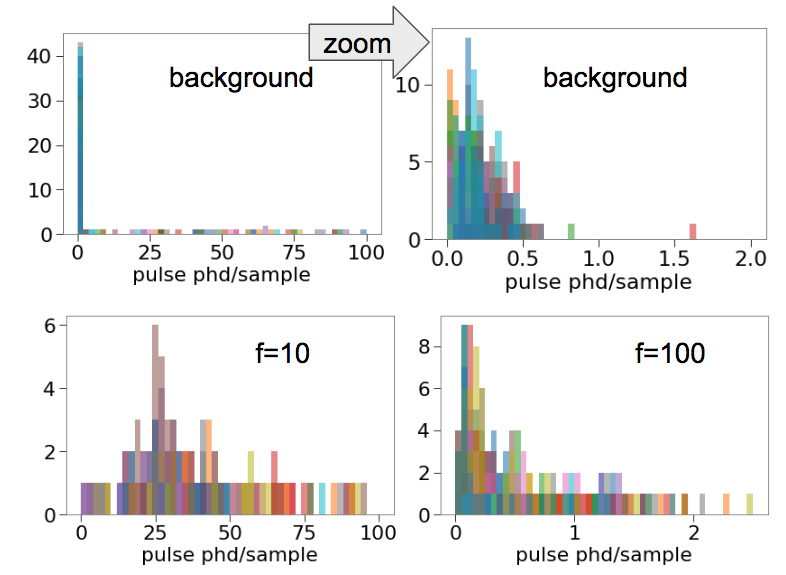
\includegraphics[width=\textwidth]{figures/lips/energy_distribution_lip_bkg.png}
\caption{The binned phd/sample straggling histograms for several events displayed on the same axes. Each color represents a different event; the top shows the straggling of background events and the bottom shows the straggling of $f=10$ and $f=100$ events. The two background panels show the same events, but the top right plot is a zoomed-in and re-binned version of the top left plot. }
\label{fig:energy_distribution_lip_bkg}
\end{center}
\end{figure}

For each event, the 10 measurements of phd/sample are treated as coming from a Moyal distribution. The Moyal distribution describes the energy loss of a charged relativistic particle due to ionization \cite{Moyal1955}, and it provides a convenient closed-form approximation to the Landau distribution \cite{Cordeiro2012}. In fact, the Anderson-Darling test was fairly robust at separating \ac{LIP}s from background even if a normal distribution was used as the test distribution, but it was found that the right-skewed tail of the Moyal distribution was helpful in keeping \ac{LIP}s. The functional form for the Moyal distribution is:

\begin{equation}
%\begin{split}
f(x) = \frac{1}{\sqrt{2 \pi}s}\mathrm{exp}(-1 ( \frac{x-\mu}{s} + \mathrm{exp}(-1\frac{x-\mu}{s} )/2))
%f(y) = exp(-1 ( y + exp(-y )/(2)))/(\sqrt{2 \pi})
%\end{split}
\end{equation}
where $\mu$ is the mean and $s$ is a scale variable. Each event was ``fit'' with distribution, following the \texttt{scipy.stats.rv\_continuous} method, which doesn't do any minimization, but simply uses the mean of the observations as $\mu$ and standard deviation as $s$ and carries out the Anderson-Darling test with the observations against this ``fit'' result. An example of a Moyal and normal distribution with the same $\mu$ and $s$ are shown in Figure~\ref{fig:pdfs} for reference.

\begin{figure}[htbp]
\begin{center}
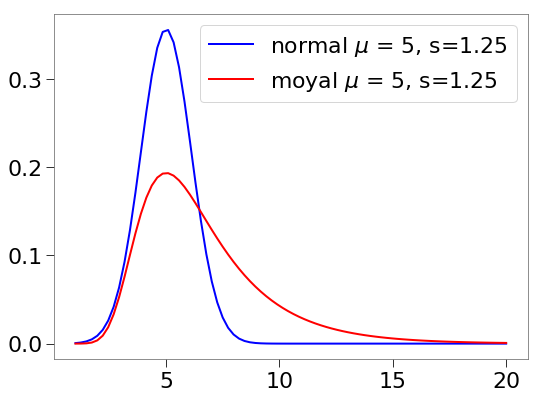
\includegraphics[width=0.6\textwidth]{figures/lips/pdfs.png}
\caption{ The Moyal and normal distributions shown for the same $\mu$ and $s$ variable. For the normal distribution $s$ is usually called $\sigma$. The Anderson-Darling test was employed for \acs{LIP}s with the Moyal as the test distribution.  }
\label{fig:pdfs}
\end{center}
\end{figure}

\FloatBarrier
\section{LIP Backgrounds}
In contrast to the \ac{WIMP} search, which throws away all multi-scatter events as background, the \ac{LIP} search must keep these events as possible signal. One origin of such events are radioactive gamma backgrounds that can multiply scatter in the detector. A detailed study of the radioactive backgrounds was completed by B. Tennyson \cite{Tennyson2017} for the Run03 detector conditions. Prior to Run03, each detector component, including the xenon itself, was counted to asses the contamination from radioactive materials. A simulation was carried out by B. Tennyson using LUXSim with initial input from the counting campaign, and subsequently adjusted to match the observed backgrounds during Run03. The output from this simulation contained 10-100 times more events than would have been observed in the \ac{LUX} Run03 exposure \cite{Tennyson2017}. The simulations showed that the maximum number of scatters a gamma underwent in the detector was 3. Therefore, setting a requirement of 4 pulses for the \ac{LIP} search reduces the gamma background from radioactive detector components to a negligible amount. 

The other source of backgrounds for \ac{LIP}s are the so-called ``electron trains'' that are present in dual phase \ac{TPC}s. The causes of electron trains are discussed in-depth in Chapter~\ref{ch:etrains}. Here, we just note electron trains are proportional scintillation signals the size of one or a few electrons that are observed to follow large energy depositions for $O(100)$~ms. Note that the observed time persistence is orders of magnitude longer than the typical event window in \ac{LUX}, which is 400~$\mu$s. Another phenomenon associated with electron trains in \ac{LUX} is colloquially referred to as an ``electron burp''. Electron burps are the sudden emission of $O(100-1000)$ electrons over the course of one or two event windows. In \ac{LUX}, electron burps have been observed to be constituents in the much longer electron trains \cite{Xu2016}. These electron noise phenomena are the main background for the \ac{LIP} analysis; they can result in similar numbers of pulses being found as for \ac{LIP}s and must be rejected with both track and energy-consistency \ac{RQ}s. There is an example of an electron train in Figure~\ref{fig:etrain_lip} and an electron burp in Figure~\ref{fig:eburp_lip}. 

\begin{figure}[htbp]
\begin{center}
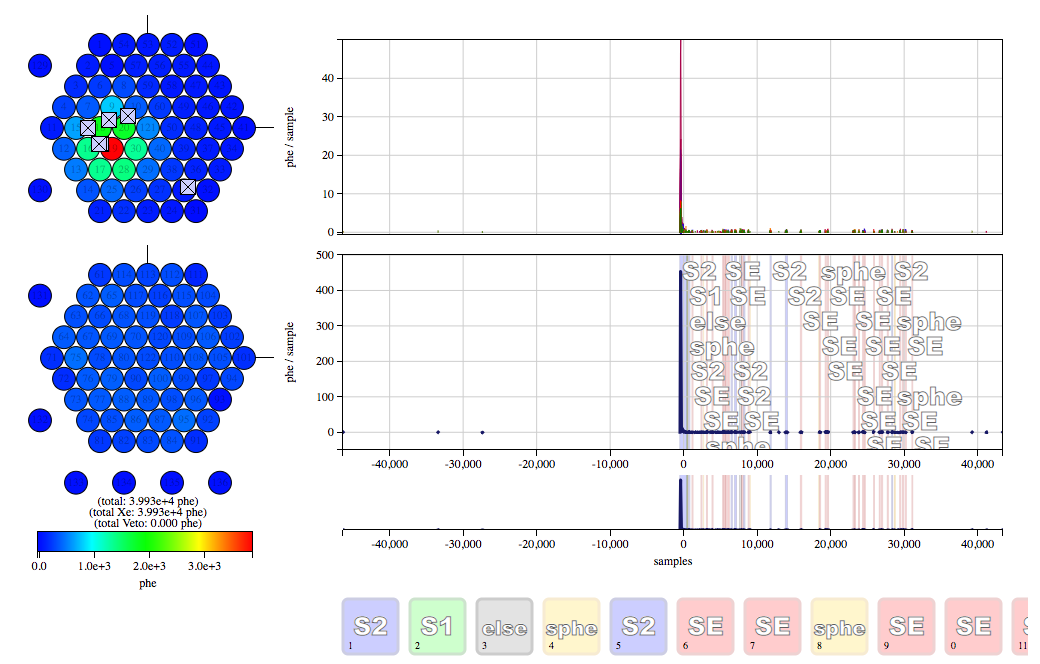
\includegraphics[width=\textwidth]{figures/lips/etrain.png}
\caption{An example of an electron train following a large S2. In this particular example, there is no S1 found before the large S2. S1s are required to provide a drift time for S2 pulses, and events with no drift time have no pulse area or position corrections applied. If only the corrected pulse areas were used, they would appear to be approximately uniform and could be confused for a \acs{LIP}. In this case, the corrected positions (displayed as ``$x$'' markers on the \acs{PMT} array) are not aligned in a track, so a track cut could reject this particular event. Sometimes, electron trains do happen to lie along a track, and \acs{RQ}s using raw S2 areas and positions must be employed. }
\label{fig:etrain_lip}
\end{center}
\end{figure}

\begin{figure}[htbp]
\begin{center}
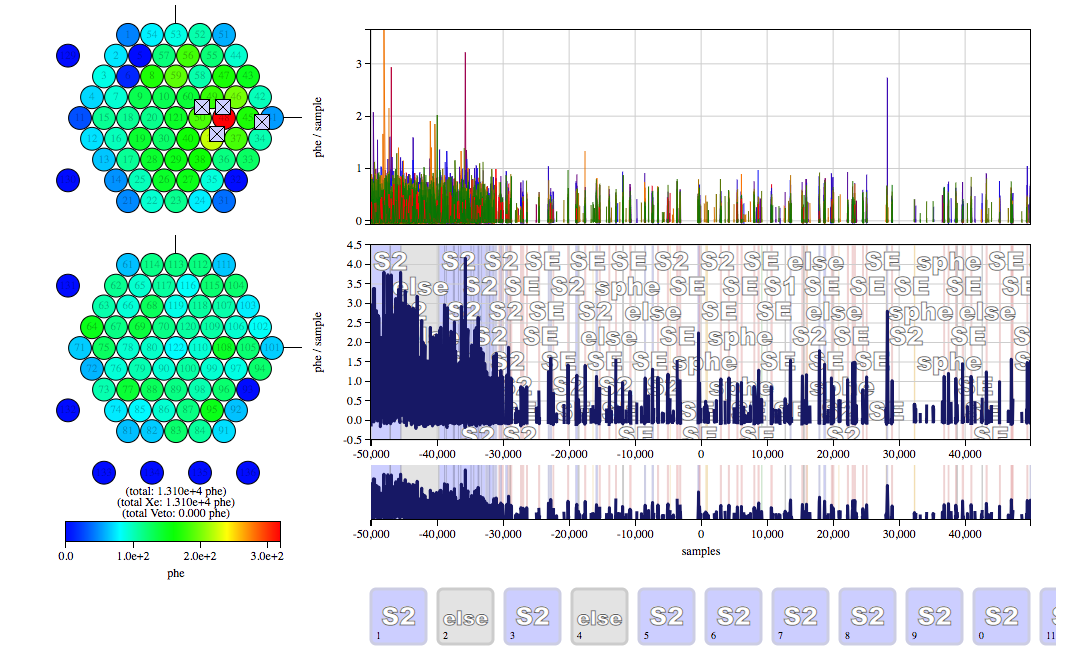
\includegraphics[width=\textwidth]{figures/lips/eburp.png}
\caption{An example of an electron burp, which happens to straddle two event windows. The S2s in electron burps are often similarly sized, and though there is no true S1, the pulse finder sometimes identifies an S1 in the midst of the electron burp. A robust method to cut these events is to limit the amount of area appearing before the S1.}
\label{fig:eburp_lip}
\end{center}
\end{figure}

Some electron background events have good track reconstruction (see Figure~\ref{fig:tracks_etrain} and Figure~\ref{fig:tracks_etrain2}). Although the track requirement is powerful in rejecting a lot of background events, other identifiers are needed to cut remaining electron backgounds. The events are displayed with the marker sizes proportional to the pulse areas to highlight how energy consistency \ac{RQ}s are useful in rejecting electron train backgrounds. Compare the electron train tracks in Figure~\ref{fig:tracks_etrain} and Figure~\ref{fig:tracks_etrain2} to the $f=100$ track reconstruction examples in Figure~\ref{fig:tracks_f100}. 

\begin{figure}[htbp]
\begin{center}
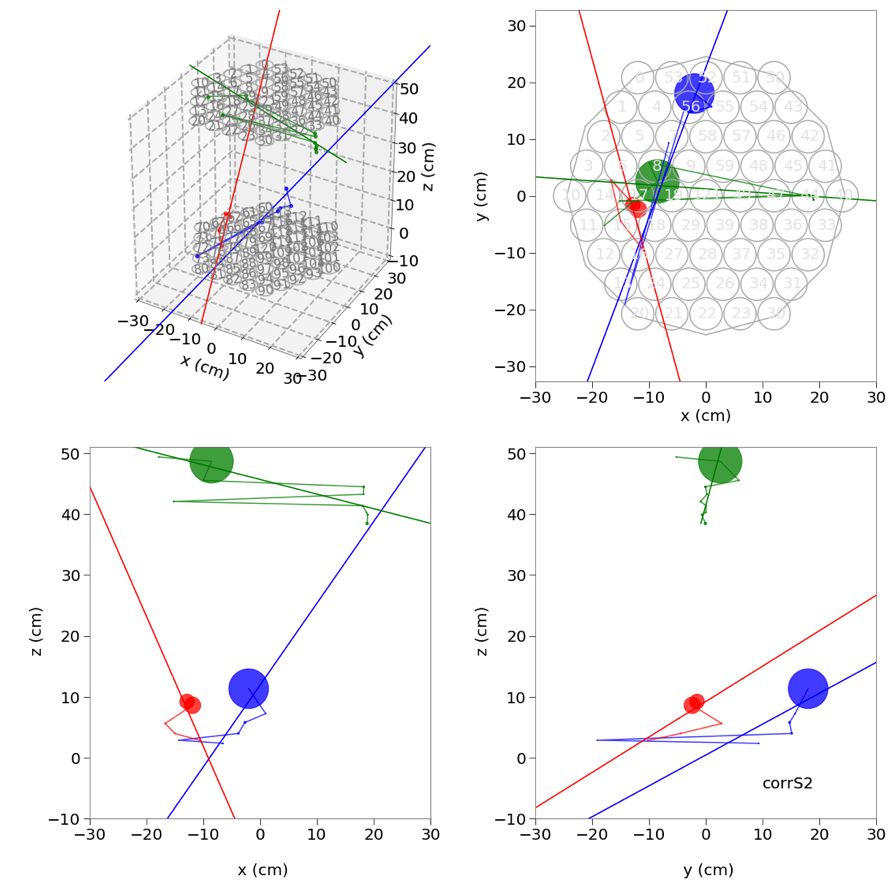
\includegraphics[width=\textwidth]{figures/lips/tracks_etrain.png}
\caption{An example of a few electron train events that led to reconstructed tracks. Different colors indicate different events. All of the 2D plots are displayed with the marker sizes scaled as pulse area. All of these events had a $\chi^{2}$ between 1.2 and 2.0. An eventual cut was applied that required $0 < \chi^{2} < 1$, so these particular events would not have made the track reconstruction cut. }
\label{fig:tracks_etrain}
\end{center}
\end{figure}

\begin{figure}[htbp]
\begin{center}
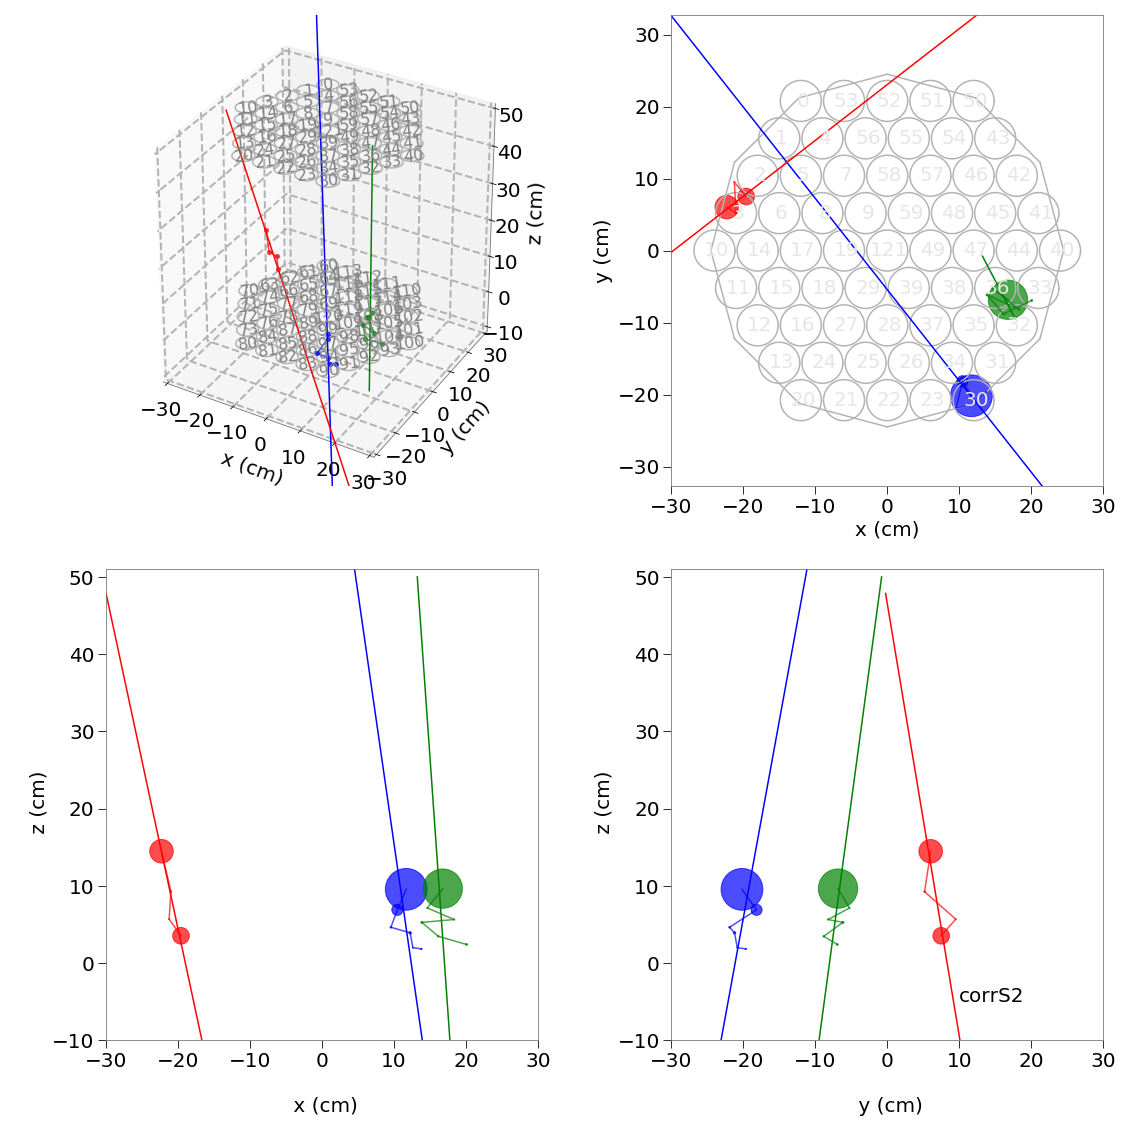
\includegraphics[width=\textwidth]{figures/lips/tracks_etrain2.png}
\caption{An example of a few electron train events that led to reconstructed tracks. Different colors indicate different events. All of the 2D plots are displayed with the marker sizes scaled as pulse area.  All of these events had a $\chi^{2} < 1.0$. An eventual cut was applied that required $0 < \chi^{2} < 1$, so these particular events would pass the track reconstruction cut. However, they do not subtend the entire detector, which we require of \acs{LIP}s. }
\label{fig:tracks_etrain2}
\end{center}
\end{figure}


\FloatBarrier
\section{LIP Search Analysis}
This section describes the analysis steps to yield a limit on the vertical flux of \ac{LIP}s observed by \ac{LUX} detector. The main \ac{LIP} background comes from delayed electron noise phenomena. Chapter~\ref{ch:etrains} summarizes the current understanding these electron noise phenomena and describes a recent study that found two distinct time scales present in electron trains. While we are getting closer to understanding the sources of electron noise, it was not extensively characterized or modeled in simulation by the \ac{LUX} collaboration. Therefore, the \ac{LIP} search lacks a background model, although a background is known to exist. The approach taken in the analysis is to develop a signal region, i.e. develop cuts with \ac{LIP} Filter \ac{RQ}s that select \ac{LIP}s while rejecting electron noise, by looking at real \ac{LUX} data. In order to avoid biasing in the cuts, only a limited amount of live data is used during cut development. This test data was not used in the final limit analysis.

\subsection{Run03 Dataset}
The analysis carried out in this section only uses about 1 month of Run03 data, with acquisitions dated from 2013-05-15 to 2013-05-31. Acquisitions within this timeframe were reprocessed using the default \ac{LUX} \ac{DPF} settings, but the number of pulses that could be found in an event was increased from 10 to 100. The total available livetime is 341.03 hours. The first 13 acquisitions, amounting to 62.56~hours, or approximately 20\% of the available data was used to develop cuts. The cuts were then carried out on the remaining approximately 80\% of the data to produce a limit on the vertical flux of \ac{LIP}s. 

\begin{figure}[htbp]
\begin{center}
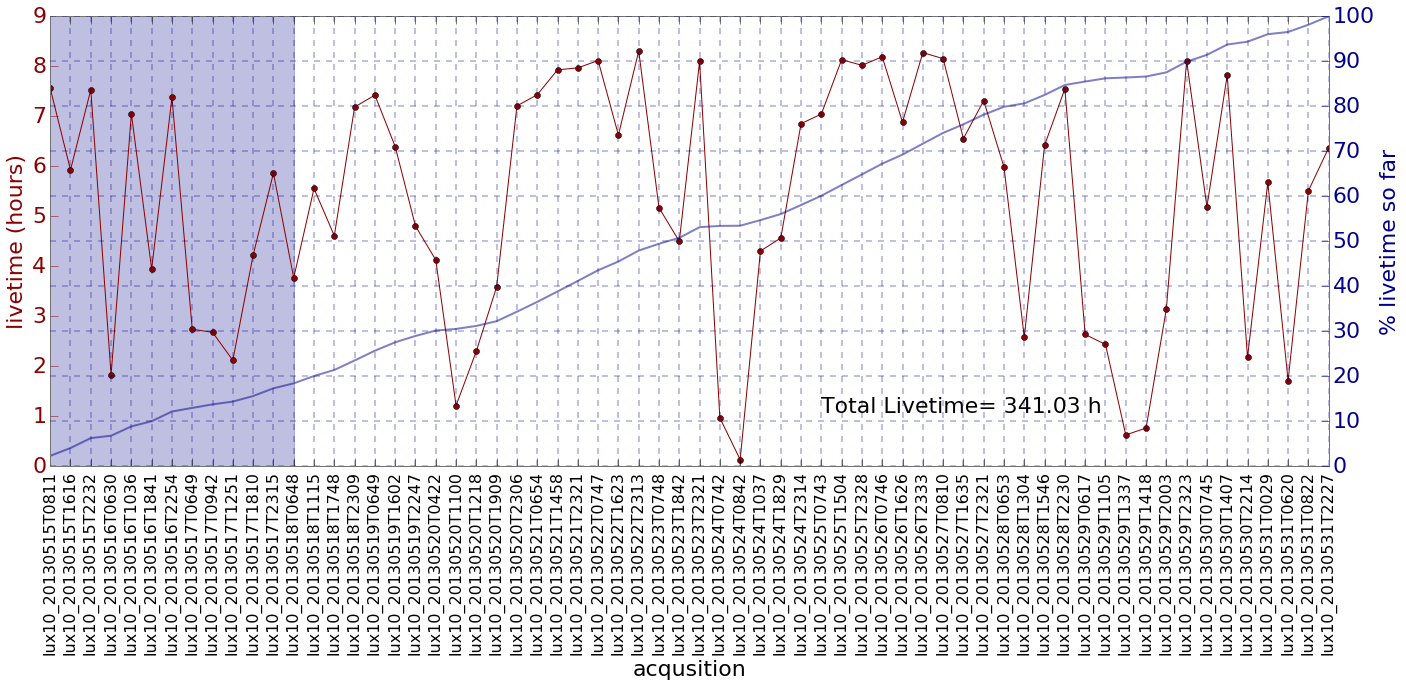
\includegraphics[width=\textwidth]{figures/lips/livetime.png}
\caption{Acquisitions from Run03 that were reprocessed, allowing 100 pulses to be found instead of the usual 10. The livetime of each acquisition is indicated in red, while the cumulative percentage of the available livetime is in blue. }
\label{fig:livetime}
\end{center}
\end{figure}

\FloatBarrier
\subsection{LIP Signal Region}
The strategy for developing the \ac{LIP} signal region cuts was to run both the \ac{LIP} simulation and 20\% of the available \ac{LUX} data through the filter. \ac{RQ}s produced by the filter were plotted side by side for \ac{LIP}s and data. If the \ac{LIP} plot displayed a somewhat compact region of signal, a loose cut was defined by the region of signal, and the cut was applied to both \ac{LIP} and data. Subsequent cuts on another \ac{RQ}s were developed similarly, and additional \ac{RQ}s were developed and tested similarly. Before applying a new cut, data events remaining in the \ac{LIP} signal regional were investigated to both assure they were not in fact \ac{LIP}s and to assess what additional cuts could be applied to eliminate the data event. Cuts were applied to both \ac{LIP} simulations and the 20\% subset of the data until no data events remained in the signal region. The efficiency for each charge fraction after all the cuts were applied to the \ac{LIP} simulation is taken to be the detection efficiency. Systematic factors affecting the efficiency are discussed in the next section, the remainder of this section shows the cuts. Each cut is illustrated with \ac{LIP} simulation on the left and data on the right.

The first cut applied is the requirement that there are more than 4 corrected S2 pulses found in the event. That is, there are 4 S2s which had successful Mercury position reconstruction, and both pulse area and position corrections were applied. The number of corrected S2 pulses is shown against the sum of all (raw) pulse area in Figure~\ref{fig:cut0}. This cut yields one of the largest losses in efficiency because there was no restriction placed on the \ac{LIP} tracks that were injected into LUXSim; there are a number of events that clip the corners of the detector, and do not have a long enough path length to produce the required number of S2 pulses. Had such a cut been placed on the injected \ac{LIP} tracks, it would have been accounted for in the calculation of $\Omega$; instead it is accounted for at this step. See Figure~\ref{fig:test_flux} for the expected rate of good S2 pulses as a function of charge fraction. For this plot, the flux is assumed to be $\Phi$ = 1/\ac{LUX}/day for all charge fractions and an overall drop from, e.g. corner clipping events is visible. 

\begin{figure}[htbp]
\begin{center}
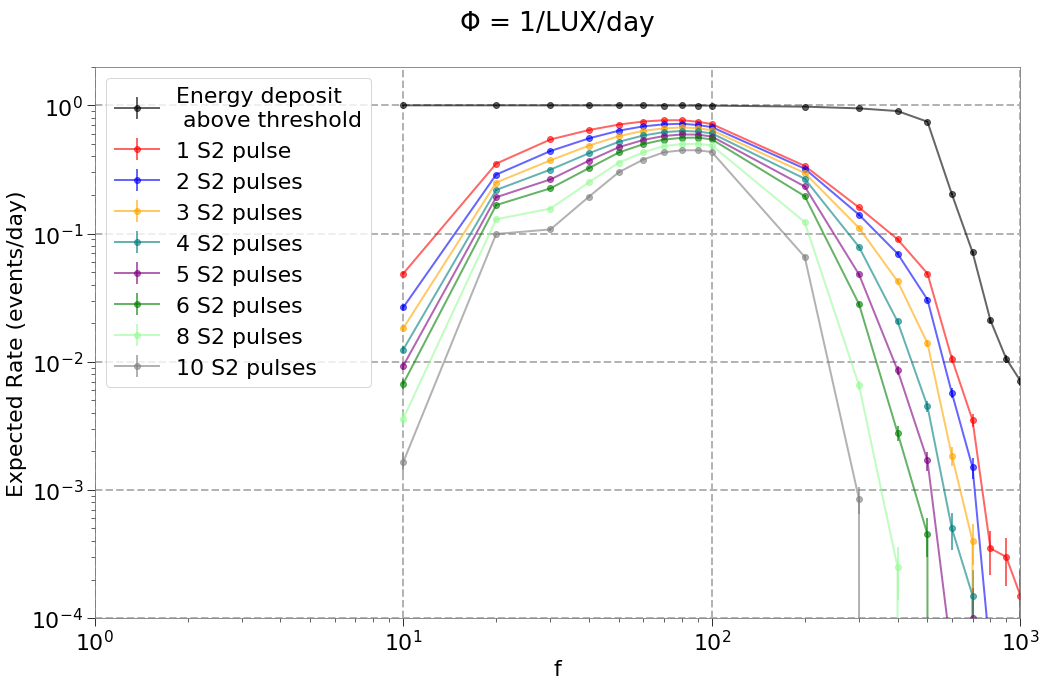
\includegraphics[width=\textwidth]{figures/lips/test_flux.png}
\caption{A plot of the expected rate of number of S2 pulses as a function of charge fraction. The flux for all charge fractions is assumed to be  $\Phi$ = 1/\ac{LUX}/day. As the charge fraction increases, the expected rate of events (black) decreases because only some events will deposit enough energy to be above threshold to trigger the detector. The fall-off is more severe when a certain number of well-reconstructed S2 pulses is required. }
\label{fig:test_flux}
\end{center}
\end{figure}


The second cut applied is the requirement that $0 < \chi^{2}/dof < 1$. The  $\chi^{2}$ used for the track fit is shown in Equation~\ref{eq:chi2}, and only S2s with successful Mercury reconstruction and position corrections are used in the track fit. This cut is shown in Figure~\ref{fig:cut1}. The third cut is a measure of whether the track subtends the entire data. The distance from the first corrected S2 position to the last corrected S2 position ($L_{data}$) is compared to the reconstructed track length from the fit ($L_{fit}$). We require $L_{fit}/L_{data} \approx 1$. Since there is no guarantee that the \ac{LIP} deposits enough energy immediately upon entering the xenon space to produce an S2, $L_{data}$ is likely always less than $L_{fit}$; this is why the cut is shifted to the right instead of being centered around 1.0. This cut is shown in Figure~\ref{fig:cut2}. The fourth cut is a a requirement that the energy depositions not vary widely as the overall energy deposition increases. The logarithm of the standard deviation in corrected S2 area is plotted versus the reconstructed S2 energy deposition per fit track length. This cut is shown in Figure~\ref{fig:cut3}. The fifth cut, shown in Figure~\ref{fig:cut4}, plots the logarithm of the standard deviation of the S2 areas versus the first two S2 pulse areas divided by the last two S2 pulse areas. For \ac{LIP}s, it is expected that the first two S2 areas are nearly identical in size to the last two S2 areas; background events show much bigger or smaller ratios, along with larger or smaller standard deviation of the S2 pulse areas. The sixth cut, shown in Figure~\ref{fig:cut5}, requires that the incident polar angle be greater than 20~degrees. A common background pathology is an event with a raised baseline in one or a small clustered group of \ac{PMT}s, along with an electron train. This background reconstructs as a vertical-going \ac{LIP} track. Since the acceptance of \ac{LUX} for vertical-going \ac{LIP}s is small, we can place a cut on incident polar angle without losing a large fraction of \ac{LIP} events. The seventh cut, shown in Figure~\ref{fig:cut6}, is similar to the \ac{LUX} ``bad area cut.'' The usual \ac{LUX} bad area cut is a limit on the amount of pulse area in an event that is not in S2 pulses -- this cuts events with a lot of electron noise. In the \ac{LIP} analysis, an S1-normalized bad area cut is placed, by plotting the raw S2 area divided by S1 area versus the corrected S2 area divided by S1 area. The ratio should be approximately 1:1 for good \ac{LIP} events; however, an efficiency loss for $f$ from about 10-50 is observed, as these events have a fair amount of area partitioned in raw S2 pulses which failed Mercury reconstruction. The efficiency is already poor for is range of charge fraction, so the loss of these events is not dramatic. Note that this cut doesn't place a requirement on the number of Else or SE in the event, which the usual \ac{LUX} bad area cut does. The eighth cut, shown in Figure~\ref{fig:cut7}, is a cut on the standard deviation between successive points on the \ac{LIP} track. The stochastic straggling and the pulse finder cause variation in the distances between the \ac{LIP} energy depositions, so some spread is expected. A common background pathology was an S2 on one side of the detector, and some electron noise occurring on the other side of the detector. Placing a cut on standard deviation of the point distances was robust is eliminating these backgrounds. The ninth and tenth cuts are both shown in Figure~\ref{fig:cut8}. A restriction is placed on the Anderson-Darling test statistic and also on the amount of area allowed in the event before the first S1. The former requires an Landu-like energy straggling and the latter is effective in cutting electron noise events. 


\begin{figure}[htbp]
\begin{center}
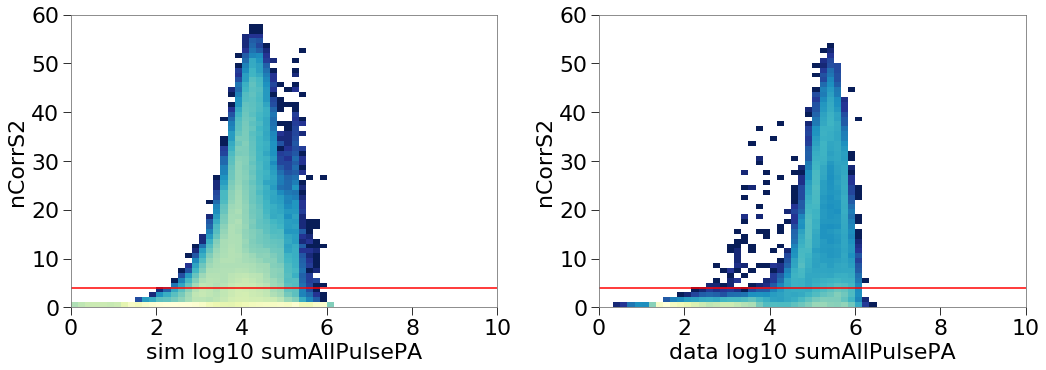
\includegraphics[width=\textwidth]{figures/lips/cut0.png}
\caption{ A 2D histogram of number of corrected S2 pulses versus the sum of all pulse area in the event. A cut is placed requiring the number of S2 pulses to be greater than 4. Only the first acquisition, lux10\_20130515T0811\_cp26812, is plotted for the demonstration.}
\label{fig:cut0}
\end{center}
\end{figure}

\begin{figure}[htbp]
\begin{center}
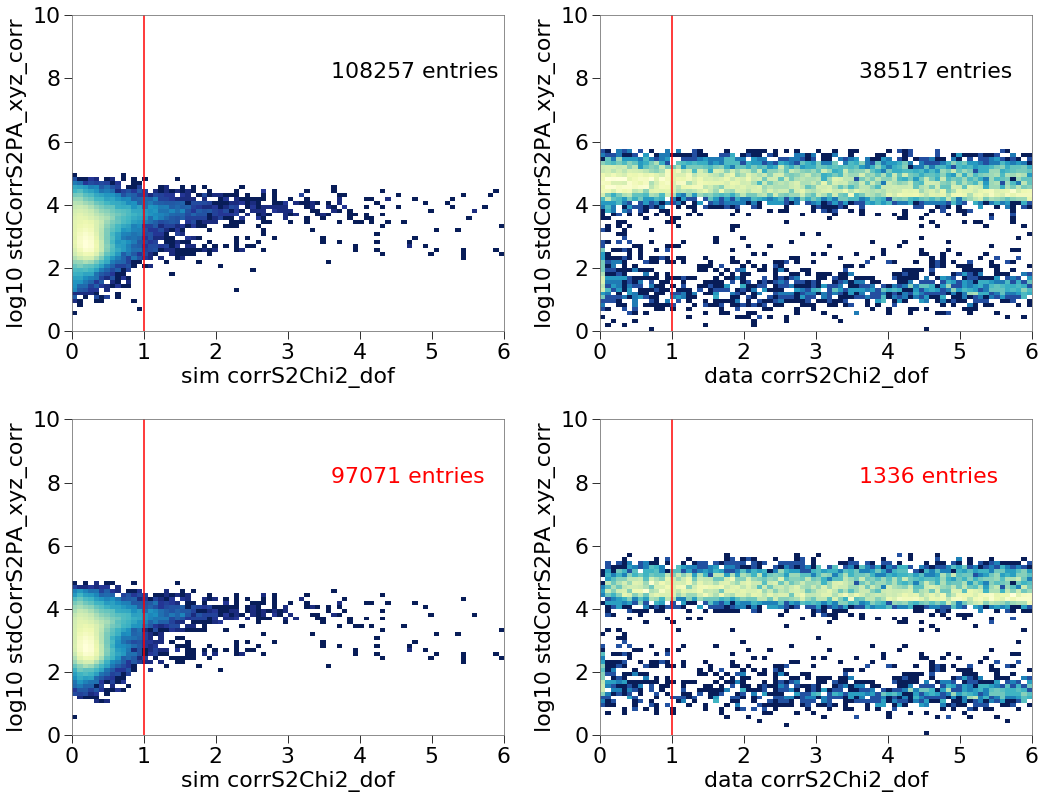
\includegraphics[width=\textwidth]{figures/lips/cut1.png}
\caption{A 2D histogram of the standard deviation of the corrected S2 pulse area versus the $\chi^{2}/dof$ from the track fit. A cut is placed requiring  $0 < \chi^{2}/dof < 1$. The top plots are shown with no cuts, the bottom plots are shown with the previous cut applied, the counts in red indicate how many events will be left after this cut. Only the first acquisition is plotted for the demonstration, all \acs{LIP} charge fractions are shown. }
\label{fig:cut1}
\end{center}
\end{figure}

\begin{figure}[htbp]
\begin{center}
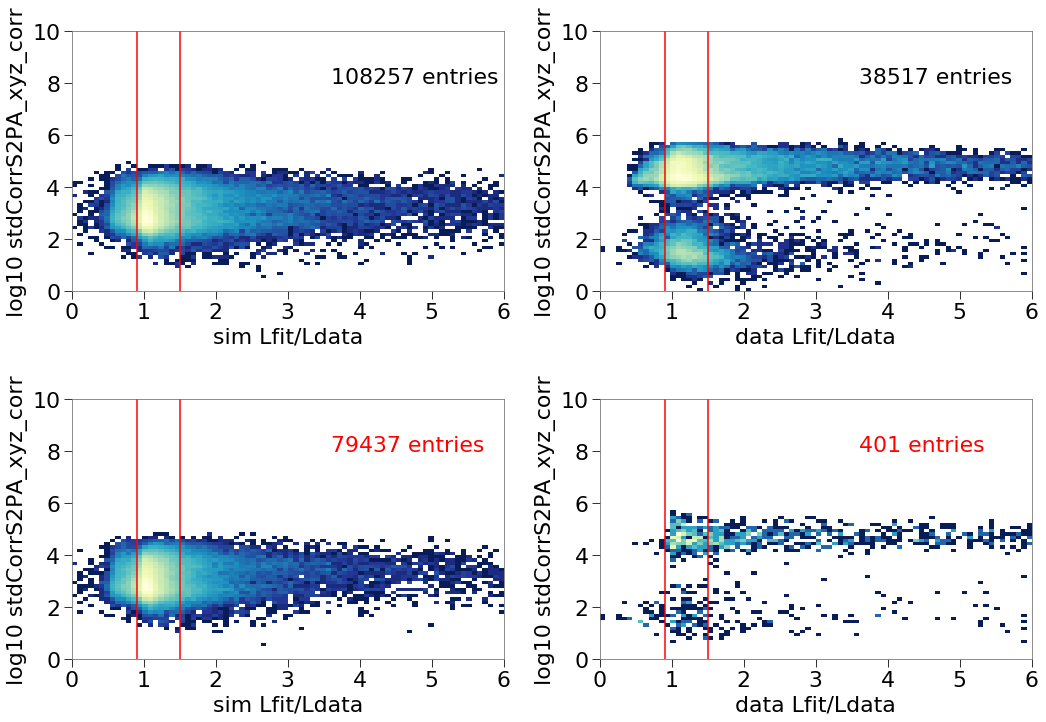
\includegraphics[width=\textwidth]{figures/lips/cut2.png}
\caption{ A 2D histogram of the standard deviation of the corrected S2 pulse area versus the fit length divided by the ``data length''. The fit length $L_{fit}$ is the reconstructed track length. The data length $L_{data}$ is defined as the distance between the first and last (corrected) S2 positions. The factor $L_{fit}/L_{data}$ is a measure of whether the event subtends the detector. A cut is placed requiring  $0.9 < L_{fit}/L_{data}< 1.5$. In general $L_{fit}$ is expected to be larger than $L_{data}$, as the \acs{LIP} may travel some distance into the \acs{LXe} before depositing energy. The top plots are shown with no cuts, the bottom plots are shown with the previous cut applied, the counts in red indicate how many events will be left after this cut. Only the first acquisition is plotted for the demonstration, all \acs{LIP} charge fractions are shown.  }
\label{fig:cut2}
\end{center}
\end{figure}

\begin{figure}[htbp]
\begin{center}
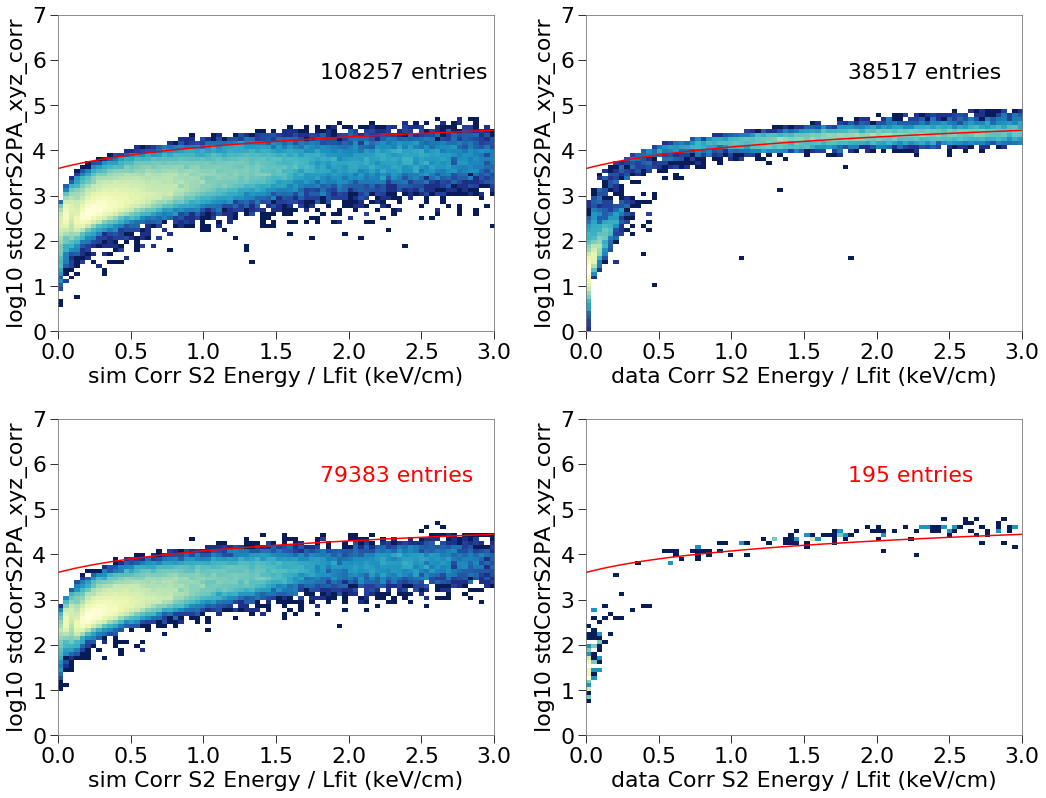
\includegraphics[width=\textwidth]{figures/lips/cut3.png}
\caption{ A 2D histogram of the standard deviation of the corrected S2 pulse area versus the corrected S2 energy divided by $L_{fit}$. The S2 energy is reconstructed using $E_{S2} = W(S2/g2)$. The top plots are shown with no cuts, the bottom plots are shown with the previous cut applied, the counts in red indicate how many events will be left after this cut. Only the first acquisition is plotted for the demonstration, all \acs{LIP} charge fractions are shown.  }
\label{fig:cut3}
\end{center}
\end{figure}

\begin{figure}[htbp]
\begin{center}
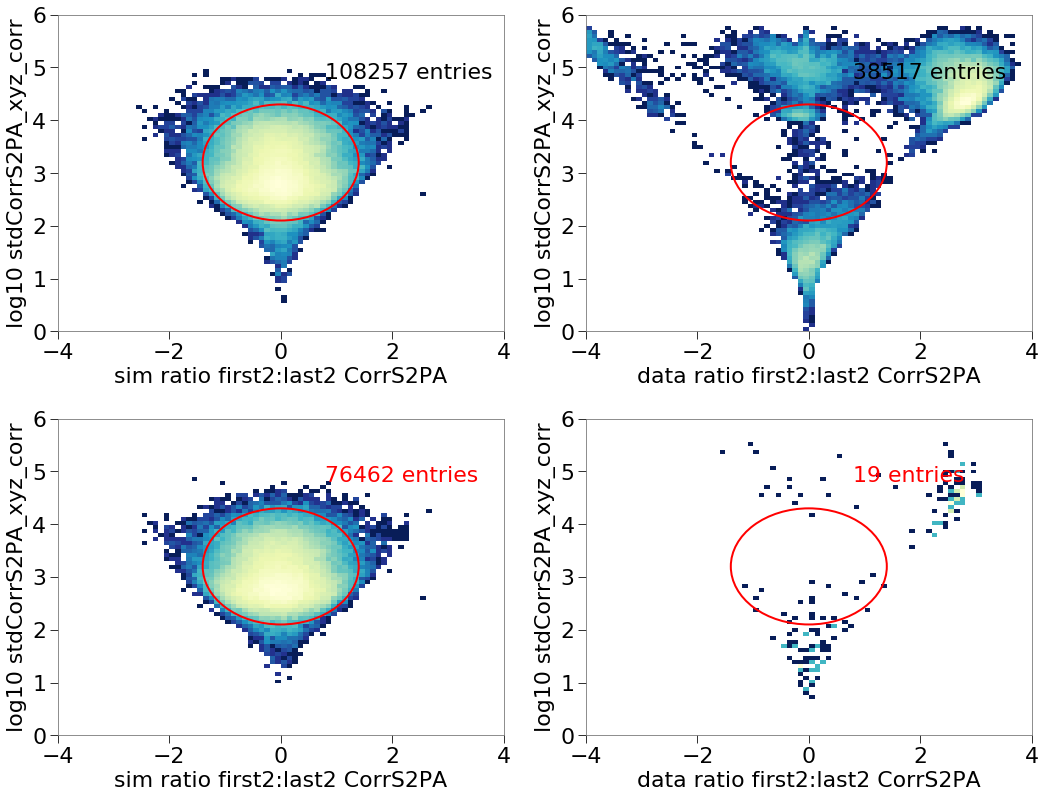
\includegraphics[width=\textwidth]{figures/lips/cut4.png}
\caption{ A 2D histogram of the standard deviation of the corrected S2 pulse area versus the ratio of the first 2 to the last 2 area corrected S2 pulses. A cut using the ellipse shown is applied. The top plots are shown with no cuts, the bottom plots are shown with the previous cut applied, the counts in red indicate how many events will be left after this cut. Only the first acquisition is plotted for the demonstration, all \acs{LIP} charge fractions are shown. }
\label{fig:cut4}
\end{center}
\end{figure}

\begin{figure}[htbp]
\begin{center}
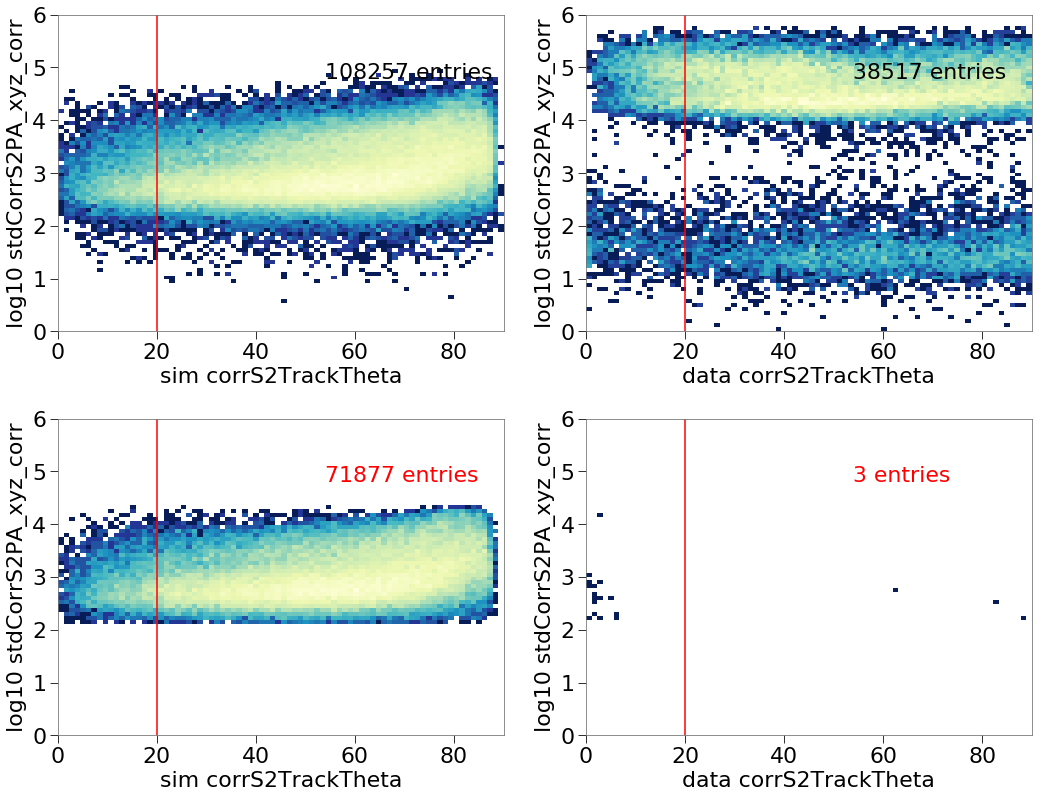
\includegraphics[width=\textwidth]{figures/lips/cut5.png}
\caption{ A 2D histogram of the standard deviation of the corrected S2 pulse area versus the reconstructed polar angle of the track. A cut requiring $\theta > 20$~deg is placed because a disproportionate number of the background electron train events appear as vertical-going \acs{LIP}s. The true acceptance for \acs{LIP}s is very limited at small polar angles, so a cut on the entry angle does not result on a large loss of signal efficiency (see Figure~\ref{fig:skymap}). The top plots are shown with no cuts, the bottom plots are shown with the previous cut applied, the counts in red indicate how many events will be left after this cut. Only the first acquisition is plotted for the demonstration, all \acs{LIP} charge fractions are shown.  }
\label{fig:cut5}
\end{center}
\end{figure}

\begin{figure}[htbp]
\begin{center}
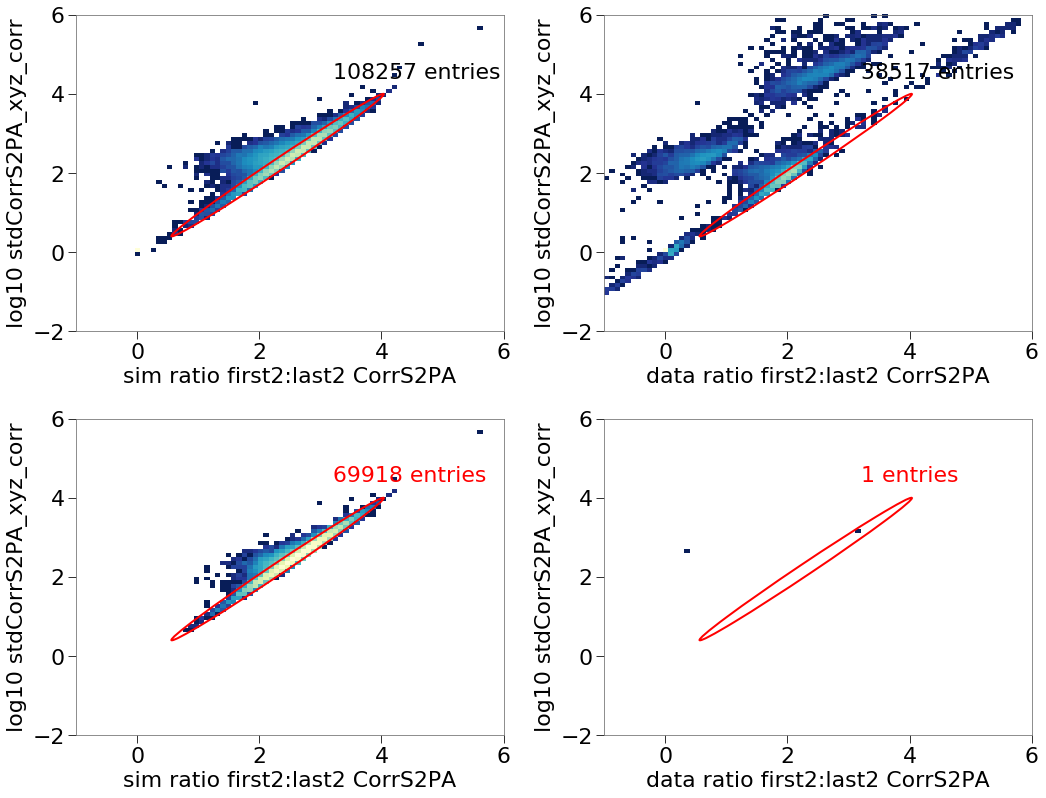
\includegraphics[width=\textwidth]{figures/lips/cut6.png}
\caption{ A 2D histogram of the raw S2 pulse area normalized to the first S1 area versus corrected S2 pulse area normalized to the first S1 area. A cut requiring events to be inside the indicated ellipse is applied. This is essentially an ``S1-normalized'' bad area cut, requiring that the pulse area in the event mostly goes into S2 area that has successful position reconstruction. The area that is being cut in the \acs{LIP} plot is loss in lower $f$, where some area is partitioned into raw S2. The top plots are shown with no cuts, the bottom plots are shown with the previous cut applied, the counts in red indicate how many events will be left after this cut. Only the first acquisition is plotted for the demonstration, all \acs{LIP} charge fractions are shown. }
\label{fig:cut6}
\end{center}
\end{figure}


\begin{figure}[htbp]
\begin{center}
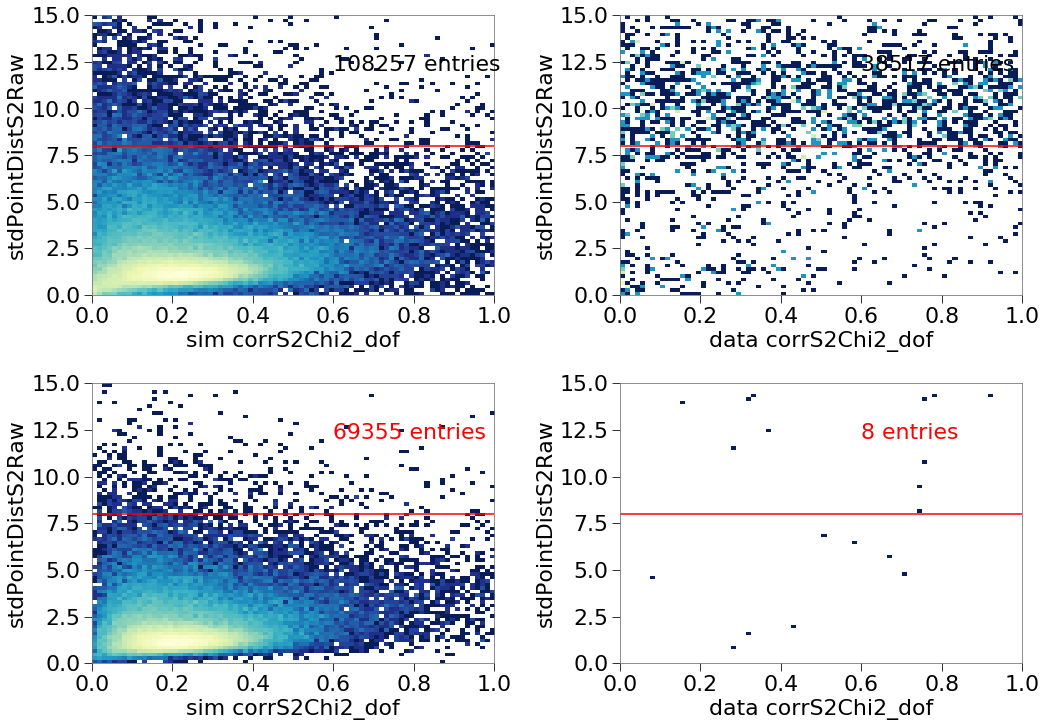
\includegraphics[width=\textwidth]{figures/lips/cut7.png}
\caption{A 2D histogram of the standard deviation of distances between the raw positions of S2s in an event versus the $\chi^{2}/dof$. A cut requiring the standard deviation between points to be less than 8~cm is applied. The top plots are shown with no cuts, the bottom plots are shown with the previous cut applied, the counts in red indicate how many events will be left after this cut. The top data plot shows only the first acquisition. The bottom data plot shows the remaining events in the first 13 acquisitions after previous cuts were applied. All \acs{LIP} charge fractions are shown.  }
\label{fig:cut7}
\end{center}
\end{figure}

\begin{figure}[htbp]
\begin{center}
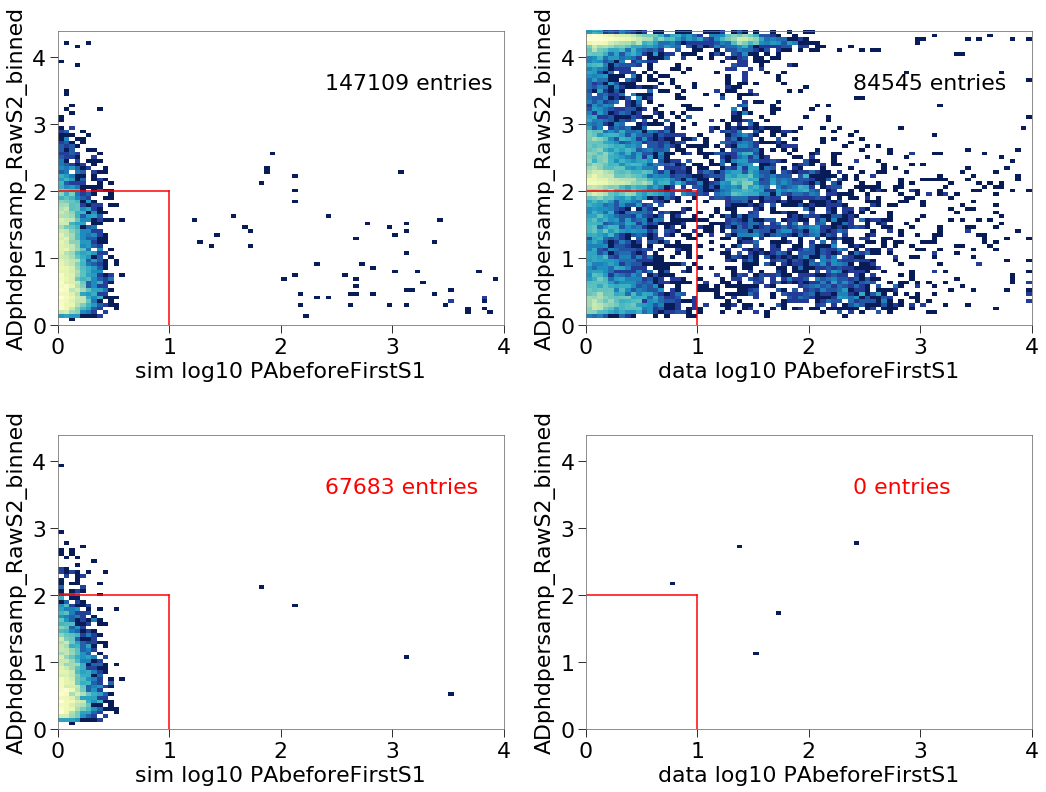
\includegraphics[width=\textwidth]{figures/lips/cut8.png}
\caption{A 2D histogram of the Anderson-Darling test statistic versus the sum of the area before the first S1. A cut is placed requiring the Anderson-Darling test statistic to be less than 2 and the area before the first S1 to fall between 0~phd and 10~phd, inclusive. The x-axis actually shows log10 of the pre-S1 area, so all events with zero area before the S1 are not shown on the plot; however, these events are retained in the cut.  The top plots are shown with no cuts, the bottom plots are shown with the previous cut applied, the counts in red indicate how many events will be left after this cut. The top data plot shows only the first acquisition. The bottom data plot shows the remaining events in the first 13 acquisitions after previous cuts were applied. All \acs{LIP} charge fractions are shown. }
\label{fig:cut8}
\end{center}
\end{figure}

The efficiency for each cut applied subsequently is shown in Figure~\ref{fig:eff}, as a function of $f$. The same cut was applied to each charge fraction, but efficiencies were calculated separately. The error bars shown are the statistical Poisson errors of how many events were within the cut region. 

\begin{figure}[htbp]
\begin{center}
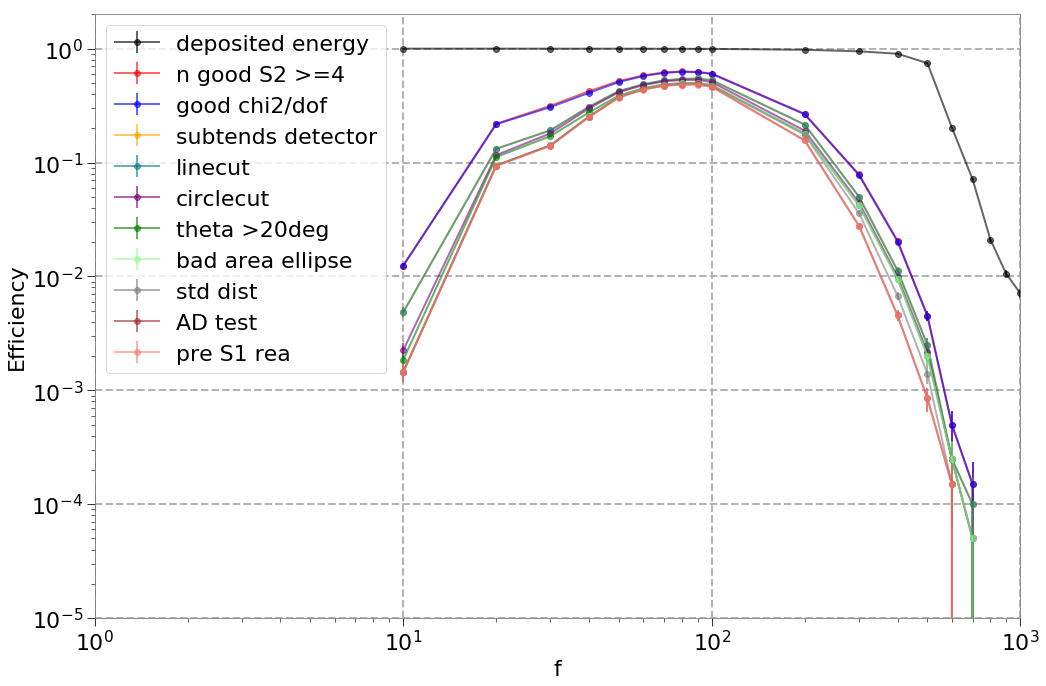
\includegraphics[width=\textwidth]{figures/lips/eff.png}
\caption{The efficiencies for each subsequent cut as a function of charge fraction. The detection efficiency is taken to be the logical and of all the cuts.}
\label{fig:eff}
\end{center}
\end{figure}

\FloatBarrier
\subsection{Systematic Errors}
\label{sec:systematics}
The base 1D straggling Monte Carlo was found to result in a measure of average energy deposition $\langle dE/dx \rangle$ 13\% less for charge fraction $f=1$ than the value given for the muon in \cite{PDG} (see Figure~\ref{fig:stochastic}). Since the detection efficiency depends heavily on track properties and not total energy deposition, the effect is expected to be small. The difference in energy deposition between two neighboring charge fractions far outweighs a 13\% increase to $\langle dE/dx \rangle$. However, the underestimation of energy deposition is a known issue, and so it was investigated. 

In order to asses the affect of the 13\% underestimation of $\langle dE/dx \rangle$ on the detection (cut) efficiency, all of the cut variables were histogrammed as a function of reconstructed energy per reconstructed path length, $E/L$. Corrected areas were used in the energy reconstruction, and path length was obtained from a fit to the corrected position variables. Any cuts in two dimensions were translated into a one dimensional cut variable. For example, the ellipse regions in Figure~\ref{fig:cut4} and Figure~\ref{fig:cut3}, were translated into the ellipse coordinates and normalized to the ellipse radius. In this manner, the cut becomes a simple one dimensional $r \leqslant 1$ cut instead of a 2D cut depending on two variables. An example of the $\chi^{2}$ variable versus $E/L$ (the stand-in for $dE/dx$) is shown in Figure~\ref{fig:chi2_dedx}. 

\begin{figure}[htbp]
\begin{center}
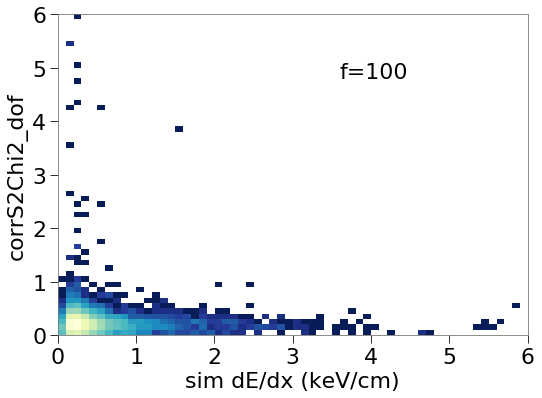
\includegraphics[width=\halffig]{figures/lips/chi2_dedx_f100.png}
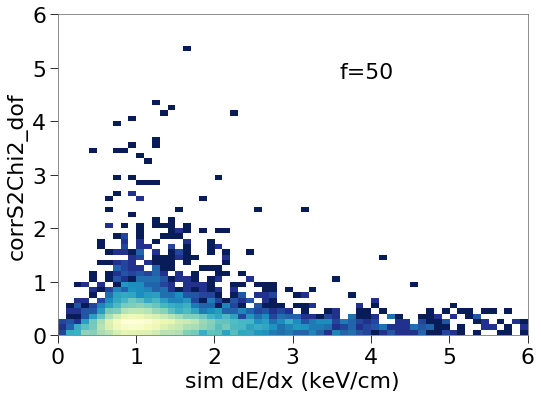
\includegraphics[width=\halffig]{figures/lips/chi2_dedx_f50.png}
\caption{ Two examples of the $\chi^{2}/dof$ dependence on $dE/dx$. The plots show the $\chi^{2}/dof$ versus the reconstructed $E/L$ for two different charge fractions. }
\label{fig:chi2_dedx}
\end{center}
\end{figure}

Histograms were constructed for each charge fraction and for all cuts discussed in the previous section, with the cut variable on the y-axis and $E/L$ on the x-axis. The $E/L$ for each event was multiplied by a factor of 1.13, and the corresponding x-bin for this new shifted valued was identified. The x-bins were not actually the equal bins shown in Figure~\ref{fig:chi2_dedx}, rather they were determined on the requirement that 5\% of the $E/L$ values were in each x-bin (see Figure~\ref{fig:chi2_dedx_bins}). Then, the y-values of the cut variable for the shifted $E/L$ bin were sampled without replacement to construct a new histogram of the cut variable versus the shifted $E/L$ (see Figure~\ref{fig:shift_example} for an example of the original and $E/L$-shifted distributions for $f=100$). The cut was applied to the new cut variable versus $E/L$-shifted distribution, and the efficiency was calculated. This procedure was done 100 times for each charge fraction. The resulting efficiencies for each cut are shown in Figure~\ref{fig:sys_eff}, where the central value is mean efficiency of the 100 trials, and the error bars are the standard deviation of efficiencies obtained from the 100 trials. This procedure was a good way to get a sense of the scale of the systematic error from placing hand-drawn cuts on populations with a known underestimation of energy, but its physical accuracy is questionable. It is unreliable to set our actual efficiency measurements to the mean of the 100 trails, but the systematic errors from this procedure is used in the limit setting.

\begin{figure}[htbp]
\begin{center}
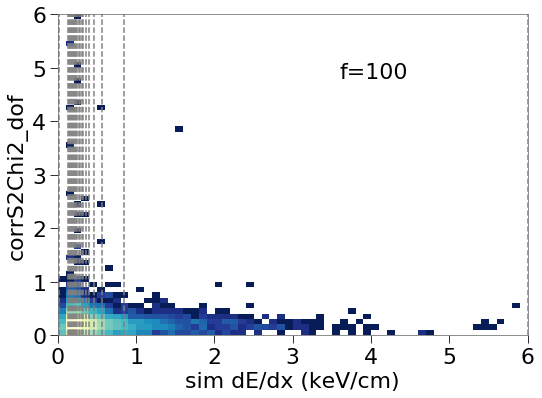
\includegraphics[width=\halffig]{figures/lips/chi2_dedx_f100_bins.png}
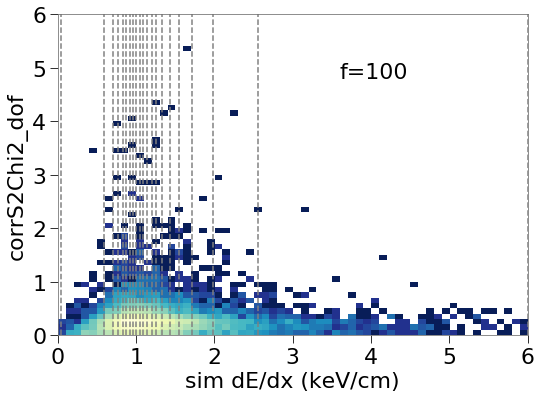
\includegraphics[width=\halffig]{figures/lips/chi2_dedx_f50_bins.png}
\caption{Examples of the 5\% bins used in the sampling procedure to asses the systematic error are overlaid (gray dotted lines) on histograms of $\chi^{2}/dof$ versus the reconstructed $E/L$ for two different charge fractions. }
\label{fig:chi2_dedx_bins}
\end{center}
\end{figure}

\begin{figure}[htbp]
\begin{center}
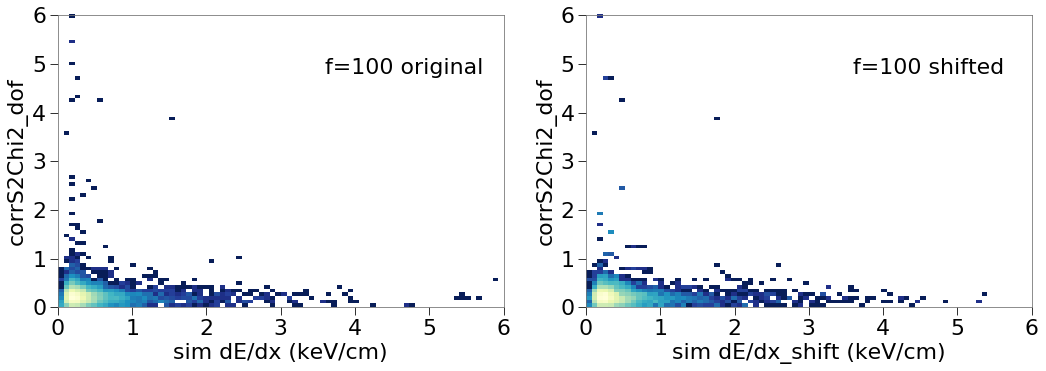
\includegraphics[width=\textwidth]{figures/lips/shift_example.png}
\caption{(left) $\chi^{2}/dof$ versus $E/L$ for $f=100$. (right) The resampled $\chi^{2}/dof$ distribution versus $E/L$ after shifting the original $E/L$ by a factor of 1.13.}
\label{fig:shift_example}
\end{center}
\end{figure}
 
 \begin{figure}[htbp]
\begin{center}
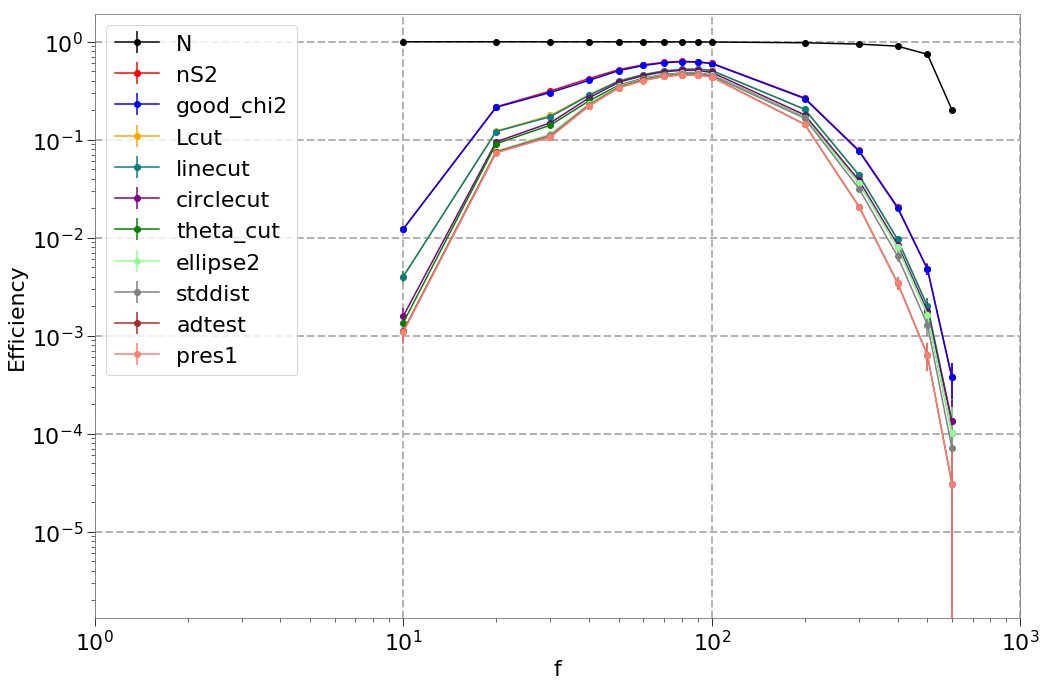
\includegraphics[width=\textwidth]{figures/lips/sys_eff.png}
\caption{The systematic efficiencies of each subsequent fit.}
\label{fig:sys_eff}
\end{center}
\end{figure}
 
 
\FloatBarrier
\section{Result: Vertical Flux Limit}
The detection efficiency is taken to be the efficiency after all cuts as in Figure~\ref{fig:eff}. The procedure described in the previous section was used to obtain systematic errors. The systematic and statistical errors are added in quadrature. The first 13 acquisitions listed in Figure~\ref{fig:livetime} (approximately 20\% of the available data) were used for cut development. Cuts were added until no data events remained in the \ac{LIP} signal region. The cuts were then carried out on the remaining 80\% of the data, with an expectation of zero background. After cuts were complete, there were zero events remaining in the signal region of the search data. Therefore, we apply the Feldman-Cousins procedure for a zero signal, zero background outcome \cite{Feldman1998}. The vertical flux limit is shown in Figure~\ref{fig:limit}.


\begin{figure}[htbp]
\begin{center}
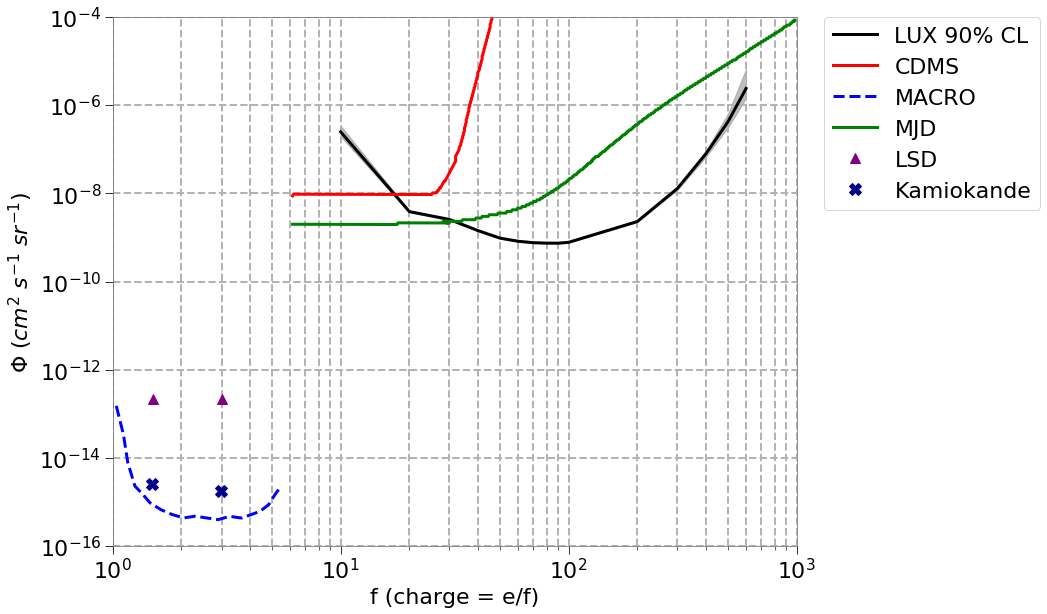
\includegraphics[width=\textwidth]{figures/lips/limit.png}
\caption{The vertical flux limit from 278.47 hours of livetime during \acs{LUX} Run03 compared to other recent flux limits. The result of this analysis is shown in black, with grey bands indicating the combined statistical and systematic error on detection efficiency.}
\label{fig:limit}
\end{center}
\end{figure}

\section{Discussion}
The flux limit presented in Figure~\ref{fig:limit} is the first of its kind from an \ac{LXe} \ac{TPC}. The range of charges probed is similar to that investigated by modern low-background cryogenic Ge detectors, but the challenges of the analysis are very different due to the phenomenon of delayed electron noise, which is the dominant background for this search. Delayed electron noise along with small energy depositions decreased the efficiency for high $f$. Charge fractions $f > 700$ deposited so little energy in the \ac{TPC}, that the ionization signals were not S2, but single electrons. Since delayed electron noise is known to continue for $O(100)$~ms, polluting subsequent events, the choice was made to require an ionization signal analysis threshold of 4 S2 pulses in an event, and reject the event if only SE ionization signals were present. Future searches could leverage better understanding of delayed electron noise and dedicated modeling and simulation of these backgrounds to extend the range of \ac{LIP} searches to higher $f$. On the other side, low $f$ events were found to deposit so much energy, creating ionization trails, that the standard data processing failed to isolate individual pulses. A modified version of data processing that, instead of attempting to find pulses, chops ionization trails into a fixed number of segments and performs the usual position and energy reconstruction on the enforced segments, would open up lower $f$ parameter space to \ac{LXe} detectors. 



%*****************************************
%*****************************************
%*****************************************
%*****************************************
%*****************************************
